This chapter describes the multicore implementation of the LM language,
including its compiler, supporting runtime and parallelism. We first start with
an overview of the implementation in order to understand how all pieces of the
implementation fit together. Secondly, we describe how parallelism is achieved,
including its data structures and thread scheduling. Thirdly, we present the
implementation details of coordination and how it relates with parallelism.  We
then describe the runtime and data structure used to implement nodes and the
database of facts, followed by the compilation algorithm used by our compiler to
turn logical rules into efficient C++ code.

\section{Overview}
The implementation of LM is composed of a compiler and a virtual machine~(VM).
Figure~\ref{fig:implementation:overview} presents an overview of the compilation
process for LM programs. The two main boxes represent the two major components
of the system, namely, the compiler and virtual machine.

\begin{figure}[ht]
  \centering
  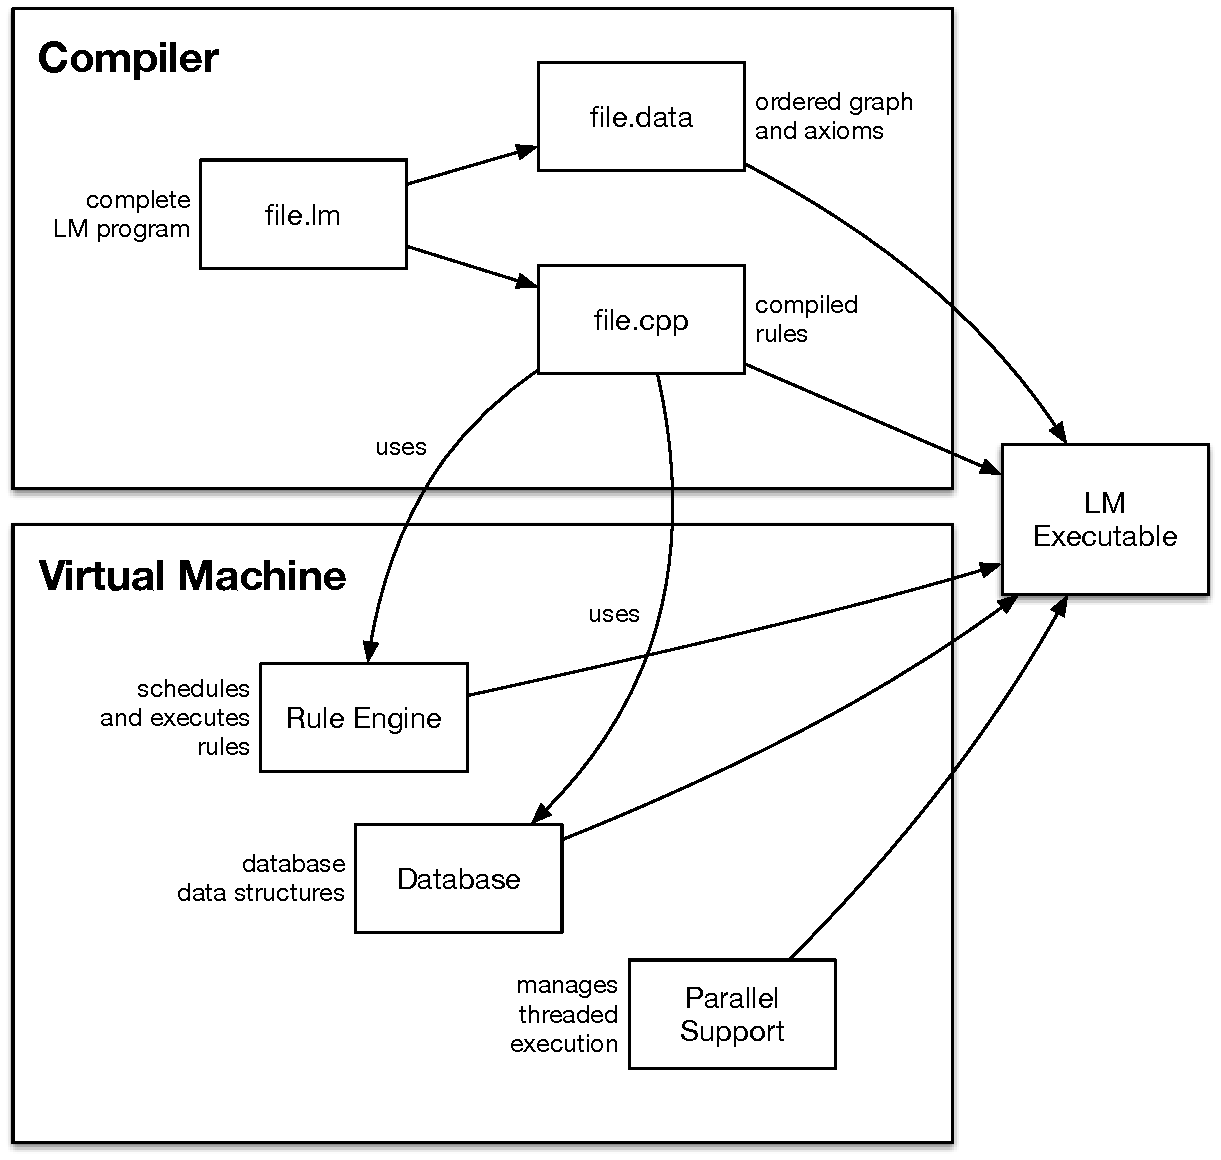
\includegraphics[width=.75\linewidth]{figures/implementation/overview.pdf}
  \caption{Compilation of a LM program into an executable. The compiler
     transforms a LM program into \code{file.cpp}, C++ file with compiled
     rules, and a \code{data} file with the graph structure and initial facts. The virtual
     machine which includes code for managing multithreaded execution and the
     database of facts is then linked with \code{file.cpp} to create a
     standalone executable that can be run in parallel.}
  \label{fig:implementation:overview}
\end{figure}

The virtual machine contains supporting data structures for managing the
database of facts and to schedule the execution of rules. The parallel engine is
also a major part of the virtual machine and is responsible for managing
multithreaded execution by launching threads, managing communication and
and scheduling parallel execution, including coordination.

The compiler transforms LM files into C++ code that use the virtual machine
facilities to implement the program logic.  The compiled code implements the
inference rules of the program and uses the API of the virtual machine to derive
and retract facts and to schedule the execution of rules.  The compiler also
creates a separate file, named \code{file.data}, with the program's initial
facts and graph structure. The graph structure is reconstructed in parallel once
the program starts.

To complete the compilation process, we use a C++ compiler to compile the
virtual machine files and \code{file.cpp} into object files that are then
linked along with \code{file.data}. At the end, we have a standalone
executable that allows the user to input the number of threads to use,
scheduling strategies (i.e., disable coordination), run time measurement
facilities and also database printing facilities.

Alternatively, the programmer may also decide to compile a more general version
of the virtual machine that is able to run byte-code files generated by the
compiler. This allows faster development since the programmer only needs to
recompile the LM program and not the whole stack. However, LM programs will run
slower since the byte-code must be interpreted by the virtual machine. This
severely affects programs with many mathematical operations, especially floating
point computations.

\iffalse
\subsection{Graph Clustering}

The graph structure stored in file \code{file.data} is constructed by the
compiler by analyzing the program's initial facts and then ordering the nodes of
the graph.  In order to distribute computation across threads it is important to
increase locality of communication, so that a node makes most of its
communication to neighbor nodes that are being handled by the same thread. The
graph structure in \code{file.data} is written in order to improve locality and
reduce communication between threads.

The compiler analyzes the node address constants (that are prepended by the
symbol @) and the initial facts of the program. After parsing and type-checking the
program code, the compiler then optimizes the topology by building an internal
representation of the graph.  In this phase, each node address $a$ is mapped
using a function $M(x)$ to a normalized node address $n$. Function $M(x)$ is
bijective and the domain is the set of all nodes described in the source code.
The co-domain of $M$ is the discrete interval $[0, N[$, where $N$ is the number
of nodes in the graph. The byte-code of a LM program includes all the pairs $(x,
M(x))$ so that the runtime system can put this information to use.

We have three methods for defining the function $M(x)$:

\begin{itemize}
   \item \emph{Static}: the compiler uses the node addresses presented in the
      code as long as they fill the discrete interval $[0, N[$.
   \item \emph{Randomized}: the mapping is done randomly.
   \item \emph{Breadth-First}: the mapping is built by picking an arbitrary node, $n_{zero}$
   and setting $M(n_{zero}) = 0$, then we select all neighbors of $n_{zero}$ and start defining
   their mappings in increasing order, $1, \dotsc, N-1$, and adding its neighbors for later processing
   in a breadth first fashion.
\end{itemize}

The breadth-first method is used with the intent of clustering closer nodes in
an ordered fashion.  While not optimal, using a breadth-first approach is very
efficient and has good results for irregular graphs. If we use a static division
of work between $N$ threads, where each thread is responsible to process a
pre-defined set of nodes, we can efficiently slice the codomain of function
$M(x)$ and divide it between the $N$ threads.

For an example, consider the graph in Fig.~\ref{fig:compiler:topology1}. The
node addresses represented are the ones included in the source code. Using a
breadth-first method starting by node 1, we get the following order: 1, 2, 3, 7,
5, 6 and 4. If we had to do a static division with 2 threads, thread 1 would get
1, 2, 3, 7 and thread 2 would get 5, 6 and 4. Note from
Fig.~\ref{fig:compiler:topology1} that only 3 edges exist between the nodes of
thread 1 and thread 2. This greatly reduces communication between threads and
improves parallel efficiency.

\begin{figure}[ht]
  \centering
  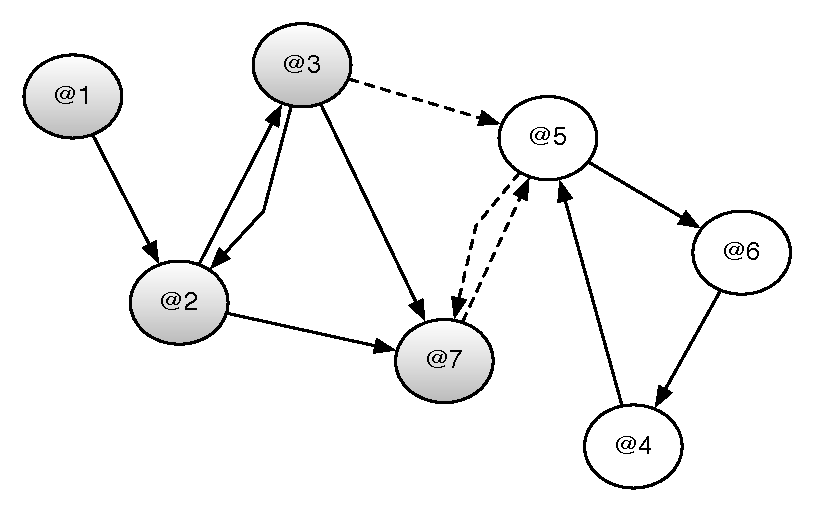
\includegraphics[width=0.6\textwidth]{figures/compiler/topology1.pdf}
  \caption{Topology using a breadth-first method.}
  \label{fig:compiler:topology1}
\end{figure}
\fi


\section{Parallelism}\label{sec:implementation:parallelism}
A key goal of our parallel design is to keep the threads as busy as possible and
to reduce inter-thread communication. Initially, the VM partitions the
application graph of $N$ nodes into $T$ subgraphs (the number of threads) and
then each thread will work on their own subgraph.  During execution, threads can
steal nodes of other threads to keep themselves busy. The load balancing aspect
of the system is performed by our work scheduler that is based on a simple work
stealing algorithm. The pseudo-code for the main thread loop is shown in
Fig.~\ref{alg:thread_work_loop}. In each round, a thread inspects its work queue
for \emph{active nodes}, which are nodes with new candidate rules and, if there
is any, procedure \texttt{process\_node()} performs computation at the node
level. If the work queue is empty, the thread attempts to steal half of the
nodes from another thread. Starting from a random thread, it cycles through all
the threads to find one active thread. Eventually, there will be no more work to
do and the threads will go idle. There is a global atomic counter, a global
boolean flag and one state flag for each thread that are used to detect
termination. Once a thread goes idle, it decrements the global counter and
changes its flag to idle. If the counter reaches zero, the global flag is set to
idle. Since every thread will be busy-waiting and checking the global flag, they
will detect the change and stop executing.

\begin{figure}
\begin{algorithm}[H]
   \KwData{Thread TH, THREADS}
   \While{true}{
      $node \longleftarrow TH.work\_queue.pop\_node()$ \;
      \uIf{$node$}{
         $TH.process\_node(node)$\;
      }
      \Else{
         \tcc{Need to steal some nodes.}
         $target \longleftarrow random(len(THREADS))$\;
         $i \longleftarrow 0$\;
         \For{$i < len(THREADS)$}{
            $target \longleftarrow (target + 1) \% len(THREADS)$\;
            $nodes = THREADS[target].steal\_half()$\;
            \If{$len(nodes) > 0$}{
               $TH.work\_queue.add\_to\_queue(nodes)$\;
               break\;
            }
            $i \longleftarrow i + 1$\;
         }
         \If{$len(TH.work\_queue) == 0$}{
            \tcc{try to terminate}
            $TH.become\_idle()$\;
            \If{$TH.synchronize\_termination()$}{
               \Return{}\;
            }
            \tcc{There's new nodes in the queue.}
            $TH.become\_active()$\;
         }
      }
 }
\end{algorithm}
\caption{Thread work loop: threads process active nodes from the work queue
   until no more active nodes are available. Node stealing using a \emph{steal
      half} strategy is employed when the thread has no more active nodes.}
 \label{alg:thread_work_loop}
\end{figure}

Figure~\ref{fig:implementation:vm_overview} presents the layout of our virtual
machine for a program with six nodes and two running threads. Each thread space
includes the nodes owned by the thread (the dotted arrows represent the edges
between nodes) and a \emph{Work Queue}, which contains \emph{active nodes},
i.e., nodes that have new facts to process, and can be implemented as a simple
linked list. Initially, the \emph{Work Queue} is filled with all the nodes of
the thread in order to derive the initial facts.
Figure~\ref{fig:implementation:vm_overview} also illustrates the internal
structure layout of a node, which includes: the database of linear facts
(\emph{Linear DB}); the database of persistent facts (\emph{Persistent DB}); the
rule matching structures (\emph{Rule Engine}); and an auxiliary buffer for
storing intermediate facts coming from other threads (\emph{Fact Buffer}).

\begin{figure*}[t]
\centering
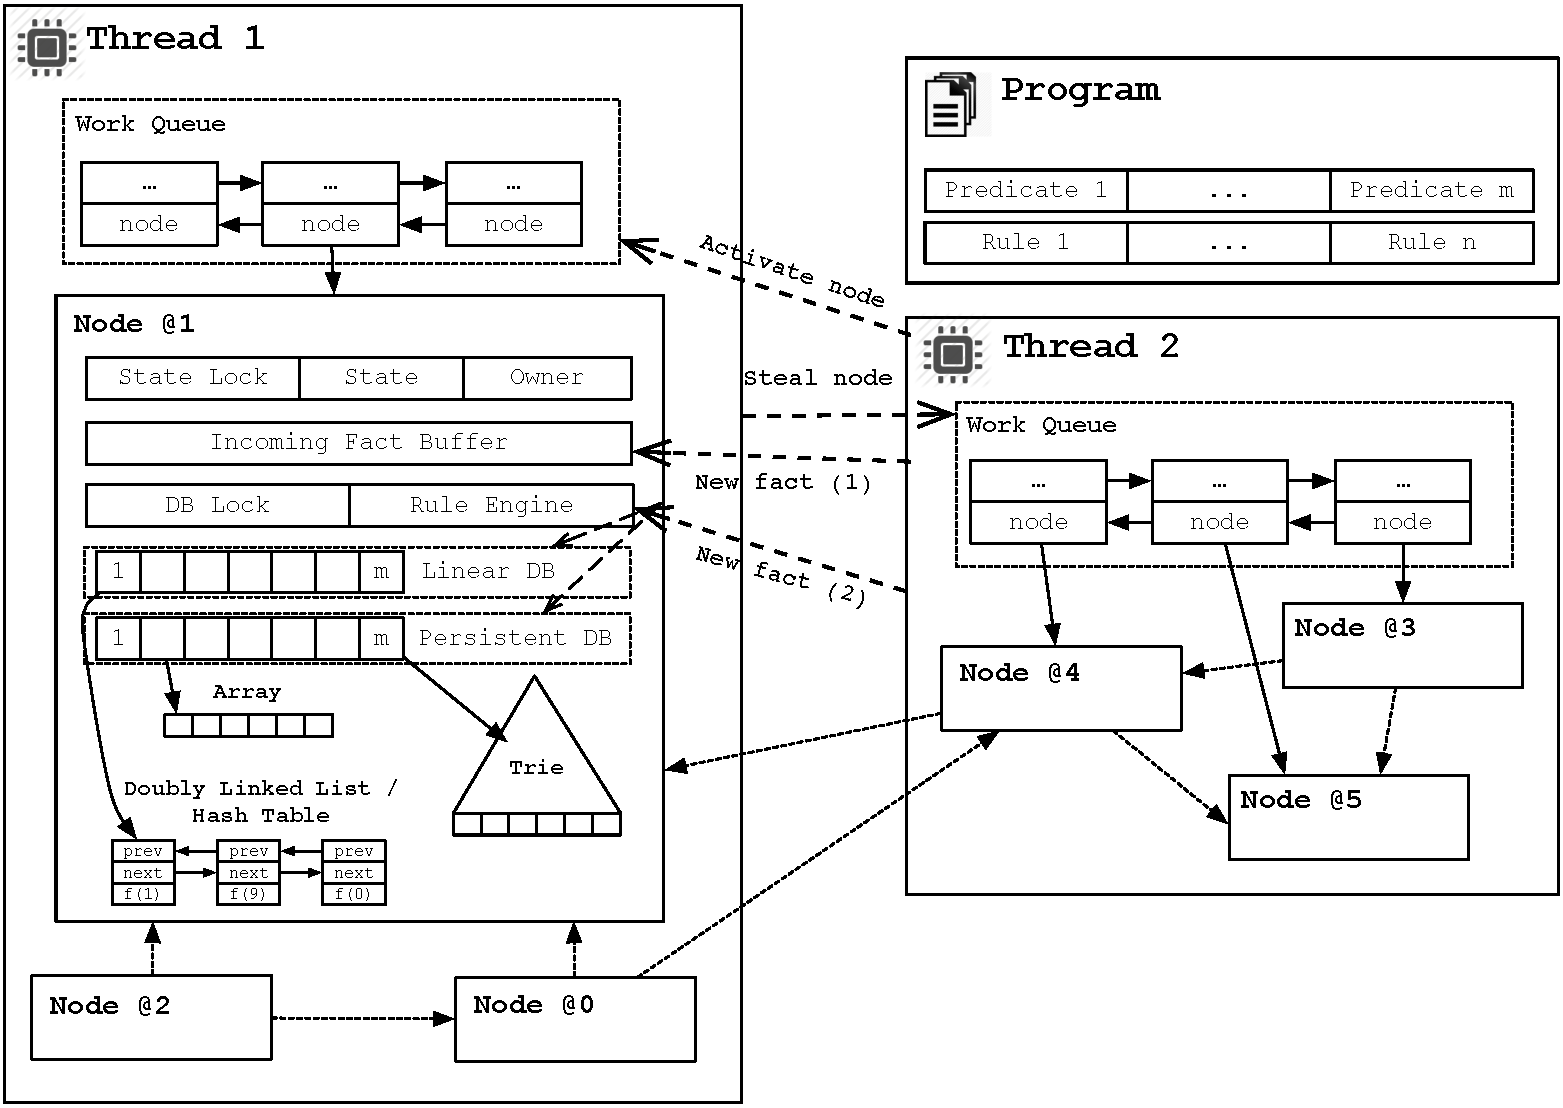
\includegraphics[width=\textwidth]{figures/implementation/vm_overview.pdf}
\caption{Layout of the virtual machine. Each thread has a work queue that
   contains active nodes (nodes with facts to process) that are processed one
   by one by the thread. Communication between threads happens when nodes
   send facts to nodes located in other threads.}
\label{fig:implementation:vm_overview}
\end{figure*}

Whenever a new fact is derived through rule derivation, we need to update the
data structures for the corresponding node. This is trivial if the thread that
derived the fact also owns the node. If that is not the case, then we have to
synchronize since multiple threads might be updating the same node's data
structures. We added a lock and a boolean flag to each node to protect the
access to its data structures. When the flag is activated, it means that the
node is currently being executed by the owning thread. For example, in
Fig.~\ref{fig:implementation:vm_overview}, if thread 2 derives a fact to node
\texttt{@1} (owned by thread 1), then thread 2 checks the node's flag and if not
activated, will lock node \texttt{@1} and perform the required updates
(\emph{New fact (1)}). If the flag is activated, it will not touch the main node
data structures, but instead will add the new fact to \emph{Fact Buffer}
(\emph{New fact (2)}). The facts stored in \emph{Fact Buffer} will then be
processed whenever the corresponding node's flag becomes active.

There is another thread interaction that might happen during fact derivation if
the node receiving a new fact is not active. In such case, the sending thread
needs to activate the node by pushing it to the \emph{Work Queue} of the target
thread. For example, consider again the situation in which thread 2 sends a new
fact to node \texttt{@1}. If node \texttt{@1} is not active, then thread 2 also
needs to activate \code{@1} by pushing it to the \emph{Work Queue} of thread 1.
After this synchronization point, the target thread is ensured to be active and
with a new node to process.

\subsection{Runtime Data Structures And Garbage Collection}

LM supports recursive types such as lists, arrays and structures. These compound
data structures are immutable and shared between multiple facts. Such structures
are stored in the heap of the VM and are managed through reference counting. For
instance, each list is a \emph{cons cell} with 3 fields: \texttt{tail}, the
pointer to the next element of the list; \texttt{head}, the element stored by
this element of the list; and \texttt{refs}, which counts the number of pointers
to this list element in the VM. The list is deleted from the heap whenever
\texttt{refs} is decremented to zero.

Nodes are also subject to garbage collection. If the database of a node becomes
empty and there are no references to the node from other logical facts, then the
node is deleted from the program. We keep around a small number of freed nodes
that can be reused immediately if another node is created.  We avoid garbage
collection schemes based on tracing since objects are created and discarded in
very specific points of the virtual machine and the runtime objects cannot
contain circular references. A reference counting mechanism is thus more
appropriate than a parallel tracing garbage collector which would entail pausing
the execution of the program to garbage collect all the unused objects.


\section{Coordination}
In order to support priorities and node partitioning, we extended the work queue
of each thread, as presented in Fig.~\ref{fig:implementation:vm_overview}, to
include two new pairs of queues: two doubly linked lists known as the
\emph{standard queue} and two min/max heaps known as the \emph{priority queue}.
The standard queue contains nodes without priorities and supports push into
tail, remove node from the head, remove arbitrary node, and remove first half of
nodes.  The priority queue contains nodes with priorities and is implemented as
a binary heap array.  It supports the following operations: push into the heap,
remove the \emph{min} node, remove an arbitrary node, remove half of the nodes
(vertical split), and priority update.  Operations for removing half of the
queue are implemented in order to support node stealing, while operations to
remove arbitrary nodes or update priority allows threads to change the priority
of nodes.  Table~\ref{fig:implementation:table_queue} shows the complexity of
queue operations and compares the standard queue against the priority queue.
Except for the remove half operation, priority queue operations are more
expensive.

\begin{table}[h]
   \begin{tabular}{| c | c | c |}
      \hline
      \textbf{Operation} & \textbf{Standard queue} & \textbf{Priority Queue} \\
      \hline
      Push & $\mathcal{O}(1)$ & $\mathcal{O}(\log{N})$ \\ \hline
      Pop & $\mathcal{O}(1)$ & $\mathcal{O}(\log{N})$ \\ \hline
      Remove & $\mathcal{O}(1)$ & $\mathcal{O}(\log{N})$ \\ \hline
      Remove Half & $\mathcal{O}(N)$ & $\mathcal{O}(\log{N})$ \\ \hline
      Priority Update & - & $\mathcal{O}(\log{N})$ \\ \hline
   \end{tabular}
   \caption{Complexity of queue operations for both the standard
      queue and the priority queue.}
   \label{fig:implementation:table_queue}
\end{table}

\begin{figure*}[t]
\centering
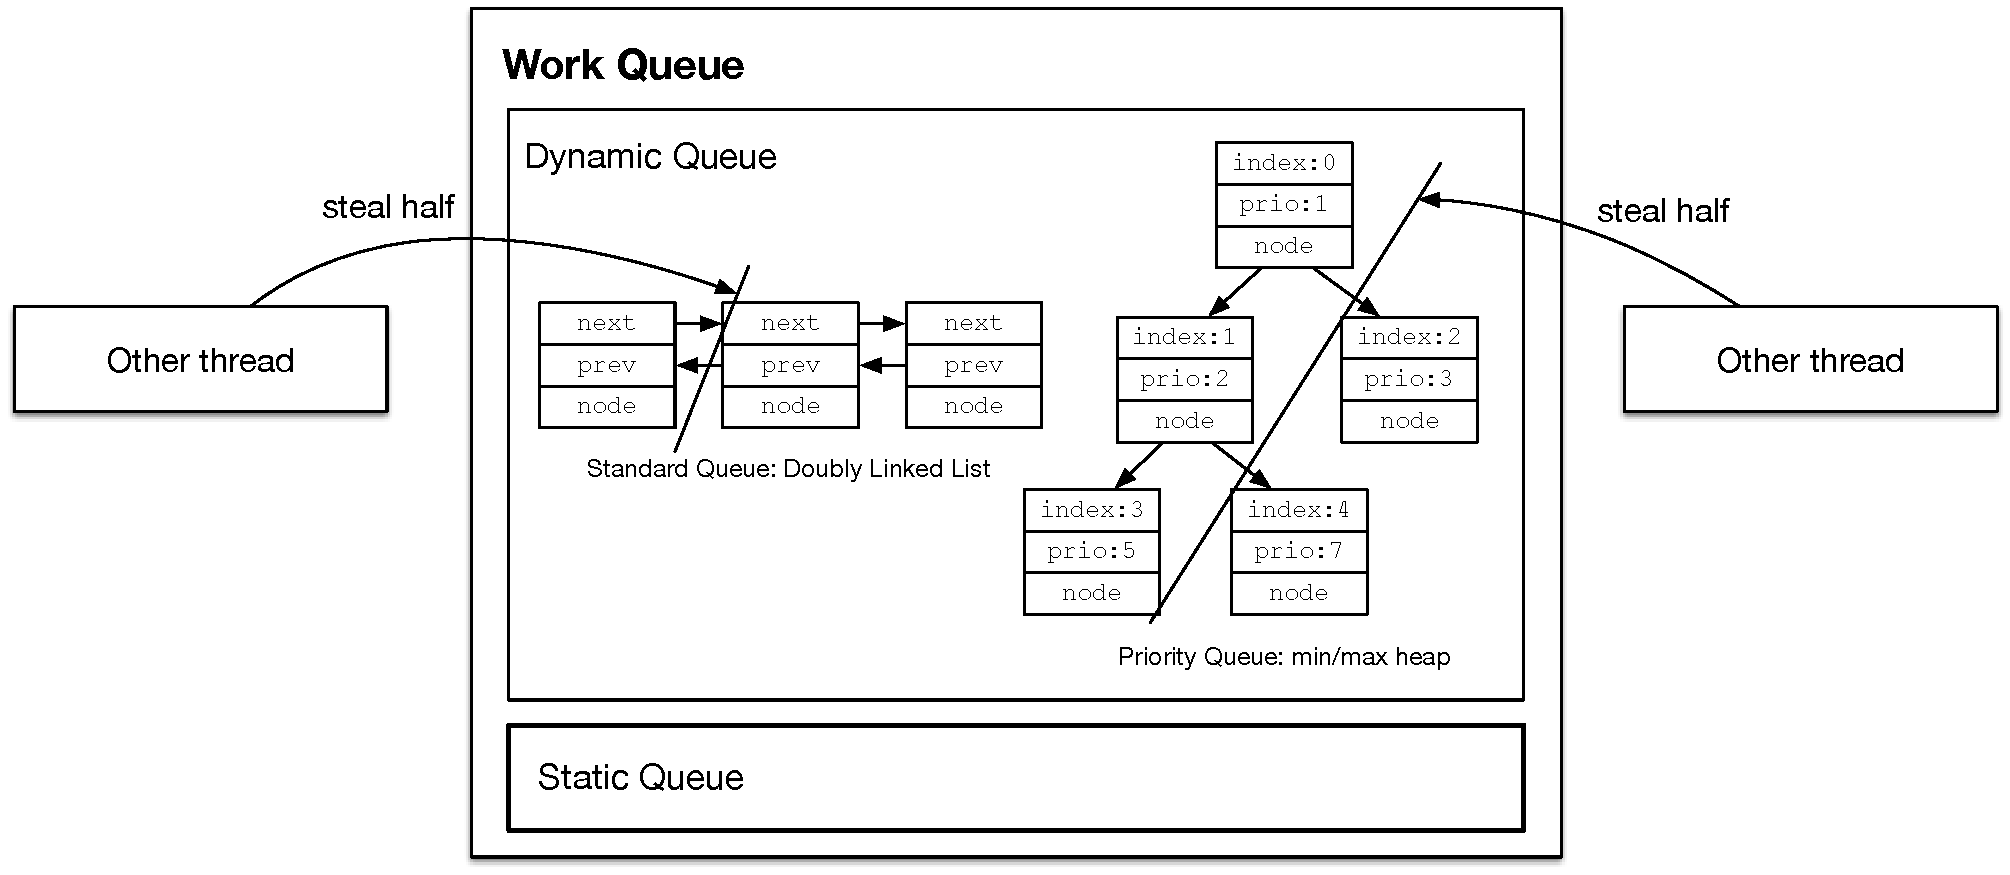
\includegraphics[width=0.95\textwidth]{figures/implementation/work_queue.pdf}
\caption{Thread's work queue and its interaction with other threads: the dynamic queue contains nodes that can be
   stolen while the static queue contains nodes that cannot be stolen. Both
   queues are implemented with one standard queue and one priority queue.}
\label{fig:implementation:work_queue}
\end{figure*}

The \texttt{next} and \texttt{prev} pointers of the standard queue are part of
the node structure in order to save space. These pointers are also used in the
priority queue but for storing the current priority and the index in the binary
heap array. Both the standard and priority queue are implemented as a pair of
queues. This first queue of each pair is a \emph{static queue} which contains
nodes that cannot be stolen and the second queue is the \emph{dynamic queue}
which contains nodes which can be stolen by other threads.
Figure~\ref{fig:implementation:work_queue} presents an overview of the two pairs
of queues and how the remove half operations are implemented in both queues in
order to support node stealing.  In the regular queue, the first $n/2$ elements
are removed from the front of the list and, in the priority queue, the binary
heap is split vertically for improved distribution of priorities.

Remember that to minimize inter-thread communication, node priorities are
implemented at the thread level, i.e., when a thread picks the highest priority
node from the priority queue, it picks the highest priority node from its
subgraph of nodes and not the highest priority node from the whole graph.

\subsection{Node State Machine}\label{sec:node_state_machine}

To accommodate the new coordination facilities, we added a new node state to the
state machine presented previously in Fig.~\ref{fig:local:node_states}.
Figure~\ref{fig:implementation:node_states} reviews the new set of states of
the state machine.

\begin{itemize}
   \item \textbf{running}: The node is deriving rules.
   \item \textbf{inactive}: The node is inactive, i.e., it has no new facts and
      it is not in any
   queue for processing.
   \item \textbf{active}: The node has new facts and it is in some queue waiting
   to be processed.
   \item \textbf{stealing}: The node has just been stolen and it is in the process of being
   moved to another thread.
   \item \textbf{coordinating}: The node moves from one queue to another or
      inside the priority queue when changing its priority.
\end{itemize}

\begin{figure}[ht]
   \centering
   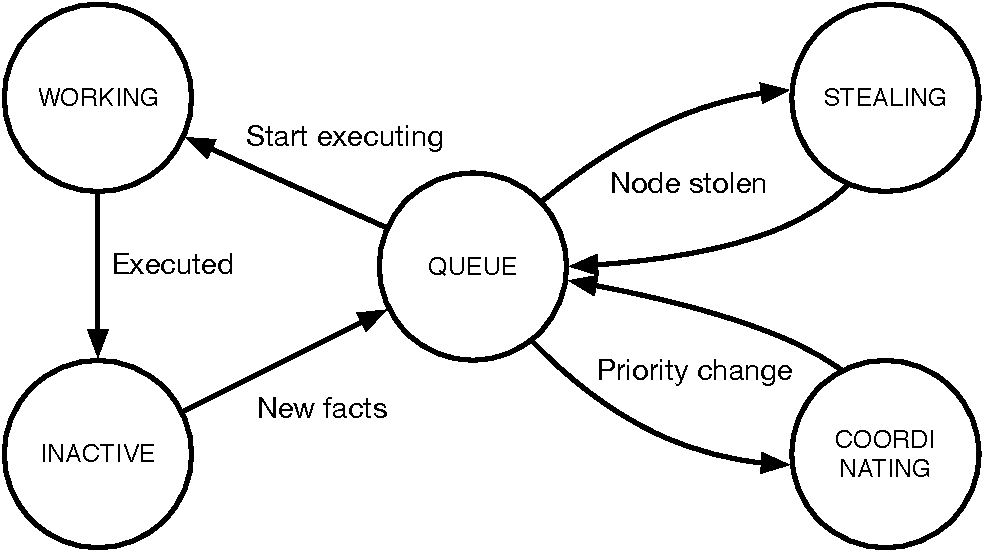
\includegraphics[width=0.55\textwidth]{figures/implementation/node_states.pdf}
   \caption{Node state machine extended with the new \textbf{coordinating}
   state.}
   \label{fig:implementation:node_states}
\end{figure}

\subsection{Coordination Instructions}\label{section:coordination:coord_instrs}

Coordination facts are implemented as API calls to the virtual machine which
implement the appropriate operations. Sensing facts read information about the
state of the virtual machine while action facts lock and update the appropriate
underlying data structures such as the node data structure or the thread's
queues.

When a thread $T_1$ performs coordination operations to a node owned by a thread
$T_2$, it needs to synchronize with $T_2$ and for that the \emph{State Lock} in
the target node needs to be acquired. Optionally, we may need to also lock the
queues of the thread $T_2$ if the priority is being updated or the queues of
thread $T_1$, if the node is moving to thread $T_1$. Note that both the standard
queue and priority queue have separate locks in order to allow concurrent
manipulation of the two data structures.

For the coordination facts \code{set-priority} and \code{add-priority}, when
multiple operations are directed to the same node during a single node
execution, we coalesce the multiple operations into a single operation.  As an
example, if a node derives two \code{set-priority} facts that change the
priority of node \code{@1} to \code{1} and \code{2}, the virtual machine
coalesces the two instructions into a single \code{set-priority} that is applied
with value \code{2} (the higher priority) after all the candidate rules of the
node are executed. The reason for this optimization is that nodes may run for
some number of steps during the lifetime of the program, therefore immediately
applying each and every coordination instruction is not cost effective. We aim
to reduce the amount of locking and movement of nodes inside the queues due to
priority updates.


\section{Thread Facts}
In the previous chapter, we introduced coordination facts, a mechanism that can
be used by the programmer to coordinate execution. While these facilities retain
the implicit parallelism of the language, they do not allow the programmer to
fully reason about the underlying parallel architecture since the only reasoning
allowed relates to node partitioning and data placement. In principle, it should
be advantageous to reason about thread state, that is, to perform rule inference
about facts stored on each thread and allow threads to communicate and
coordinate between them depending on their current state. This introduces a kind
of explicit parallelism into the implicit parallel model of LM.  However, this
explicit parallelism remains declarative so that the programmer is able to
reason thread coordination as well as it does with regular computation.

\section{Motivational Example: Graph Searching}
Consider the problem of checking if a set of nodes $S$ in a graph $G$ is
reachable from an arbitrary node $N$. An obvious solution to this problem is to
start at $N$, gather all the neighbor nodes into a list and then recursively
visit all those reachable nodes, until $S$ is covered. This reduces to a problem
of performing a breadth or depth-first search on graph $G$. However, this
solution is sequential and does not have much concurrency.  An alternative
solution to the problem is to recursively propagate the search to all neighbors
and aggregate the results in the node where the search started.  The code for
this later solution is shown in Fig.~\ref{code:threads:reach_simple}.

\begin{figure}[h]
\begin{Verbatim}[numbers=left,fontsize=\codesize,commandchars=*\#\&]
type int id.*hfill// Type declaration
type list int reach-list.

type edge(node, node).*hfill// Predicate declaration
type value(node, int).
type linear search(node, id, reach-list).
type linear do-search(node, id, node, reach-list).
type linear lookup(node, id, reach-list, int Val).
type linear new-lookup(node, id, int Val).
type linear visited(node, id).

search(A, Id, ToReach)*label#line:threads:reach_lookup1&*hfill// Rule 1: initialize search
   -o do-search(A, Id, A, ToReach),
      lookup(A, Id, ToReach, []).*label#line:threads:reach_lookup2&

lookup(A, Id, ToReach, Found), new-lookup(A, Id, Val)*hfill// Rule 2: new reachable node found
   -o lookup(A, Id, remove(ToReach, Val), [Val | Found]).

do-search(A, Id, Node, ToReach),*label#line:threads:reach_visit1&*hfill// Rule 3: node has already seen this search
visited(A, Id)
   -o visited(A, Id). *label#line:threads:reach_visit2&

do-search(A, Id, Node, ToReach),*hfill// Rule 4: node found and propagate search
!value(A, Val), Val in ToReach*hfill// New node was found.
   -o visited(A, Id),*label#line:threads:reach_visit_visited1&
      new-lookup(Node, Id, Val),
      {B | !edge(A, B) -o do-search(B, Id, Node, remove(ToReach, Val))}.*label#line:threads:reach_propagate&

do-search(A, Id, Node, ToReach),*hfill// Rule 5: node not found and propagate search
!value(A, Val), ~ Val in ToReach*hfill// Not the node we are looking for.
   -o {B | !edge(A, B) -o do-search(B, ID, Node, ToReach)},*label#line:threads:reach_propagate2&
      visited(A, Id).*label#line:threads:reach_visit_visited2&
\end{Verbatim}

\caption{LM code to perform reachability checking on a graph.}
\label{code:threads:reach_simple}
\end{figure}

Each distinct reachability search is represented by a number (\code{Id}) and a
\code{search} axiom. Associated to each search \code{Id} is a list of nodes to
reach.  The predicate \code{visited} marks nodes that have already
participated in search, while predicate \code{do-search} is used to propagate a
specific search. The first rule
(lines~\ref{line:threads:reach_lookup1}-\ref{line:threads:reach_lookup2}) starts
a particular search by deriving a \code{do-search} and an \code{lookup} fact.
The \code{lookup} fact is used as an accumulator and is stored in the starting
node. The third rule
(lines~\ref{line:threads:reach_visit1}-\ref{line:threads:reach_visit2}) avoids
visiting the same node twice in the presence of a \code{visited} fact.  This
visited fact is derived in the next two rules
(lines~\ref{line:threads:reach_visit_visited1}
and~\ref{line:threads:reach_visit_visited2}).  If the node where the search is
being performed is in the set of nodes we want to reach (\code{ToReach}) then we
remove the node value from the list and propagate the search to the neighbor
nodes (line~\ref{line:threads:reach_propagate}).  Otherwise, the search is
propagated but no value is removed from \code{ToReach}.

As an example, consider Fig.~\ref{fig:threads:reach_example}, which shows 2
reachability checks on a graph with 10 nodes. For instance, the search with
\code{Id = 0} starts at node \code{@1} and checks if nodes \code{@1}, \code{@2},
and \code{@3} are reachable from \code{@1}. Since \code{@1} is the starting
node, \code{1} is immediately removed from the reachable list, including the
propagated \code{do-search} facts but also the \code{lookup} fact that is stored
at node \code{@1}. Once \code{do-search} reaches node \code{@3}, the value
\code{3} is removed from the list and a new \code{do-search} is propagated to
node \code{@1} (not shown in the figure) and \code{@2}. At the same time, node
\code{@2} receives the list \code{[2,3]}, removes \code{2} and propagates
\code{[3]} to node \code{@3} and \code{@1}. Node \code{@1} receives two
\code{new-lookup} facts, one from \code{@3} and another from \code{@2}, due to
successful searches and the \code{lookup} fact becomes \code{lookup(@1,0,[],
[1,2,3])}.

The attentive reader will notice that node \code{@1} already knows that all the
nodes have been reached and that nodes \code{@7} and \code{@4} will, needlessly,
continue to check if \code{[2,3]} are reachable. This is an issue that arises
because the programmer has valued concurrency by increasing redundancy and
reducing communication between nodes. It would be prohibitly expensive to share
reachability information between nodes. An alternative solution is to store the
results of the search on the thread performing the search and then coordinate
the results with other threads since the number of threads is usually smaller
than the number of nodes. Before showing how the reachability program is solved
using thread-based facts, we first present the changes to the language.

\begin{figure}[ht]
\begin{center}
   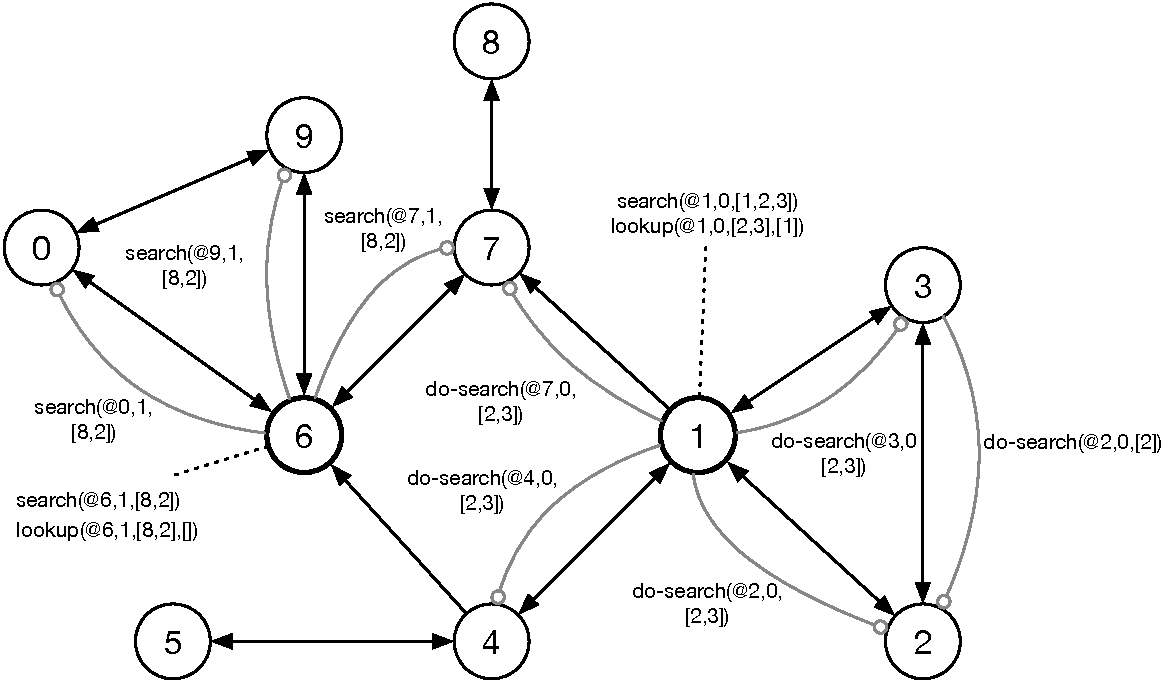
\includegraphics[width=0.9\linewidth]{figures/threads/reach.pdf}
\end{center}

\caption{Performing reachability checks on a graph using nodes \code{@1}
(\code{Id = 0}) and \code{@6} (\code{Id = 1}).  Search with \code{Id = 0} wants
to reach nodes \code{@1}, \code{@2}, and \code{@3} from node \code{@1}. Since
\code{@1} is part of the target nodes, the fact \code{do-search} propagated to
neighbor nodes does not include \code{1}.}

\label{fig:threads:reach_example}
\end{figure}

\subsection{Language Changes}

In the previous chapter, we presented coordination facts such as
\code{thread-id} and \code{set-thread} that already bring some awareness about
the underlying parallel system. Furthermore, such facts also introduce the
\code{thread} type for predicate arguments, which refers to a thread in the
system that is related to a core in a multi core processor. We now introduce the
concept of \emph{thread facts}, which are logical facts stored at the thread
level, meaning that, each thread is now an entity with its own logical facts.
The type \code{thread} is also now the type of the first argument of
\emph{thread predicates}, indicating that the predicate is related and is to be
stored in a specific thread. We also view the available threads as forming a
separate graph from the data graph, a graph of the processing units which are
operating on the data graph.

The introduction of thread facts increases the expressiveness of the system in
the sense that it is now possible to write inference rules that reason about the
state of the threads. This creates optimization opportunies since we can now
write algorithms with global information stored in the thread, while keeping the
LM language fully declarative. Moreover, threads are now allowed to explicitly
communicate with each other, and in conjunction with coordination predicates,
enable the writing of complex scheduling policies.

We discriminate between two new types of inference rules. The first type is the
\emph{thread rule} and has the form \code{a(T), b(T) -o c(T)}, and can be read
as: if thread \code{T} has fact \code{a(T)} and \code{b(T)} then derive fact
\code{c(T)}. The second type is the \emph{mixed rule} and has the form
\code{a(T), d(N) -o e(N)} and can be read as: if thread \code{T} is executing
node \code{N} and has the fact \code{a(T)} and node \code{N} has the fact
\code{d(N)} then derive \code{e(N)} at node \code{N}. Thread rules reason solely
at the thread level, while mixed rules allow reasoning about both thread and
node facts. Logically, the mixed rule uses an extra fact \code{running(T, N)},
which indicates that thread \code{T} is currently executing node \code{N}. The
\code{running} fact is implicitly retracted and asserted every time the thread
selects a different node for execution. This makes our implementation efficient
since a thread does not need to look for nodes that match mixed rules and it is
then the scheduling of the program that drives the matching of such rules.

\subsection{Graph Of Threads}

Figure~\ref{fig:coord:thread_facts} represents a schematic view of the two graph
data structures of a program with three threads: thread $T1$ is executing node
\code{@5}, $T2$ is executing node \code{@4}, and $T3$ is executing node
\code{@3}. Note that every thread has access to its own facts and to the node
facts.

\begin{figure}[ht]
   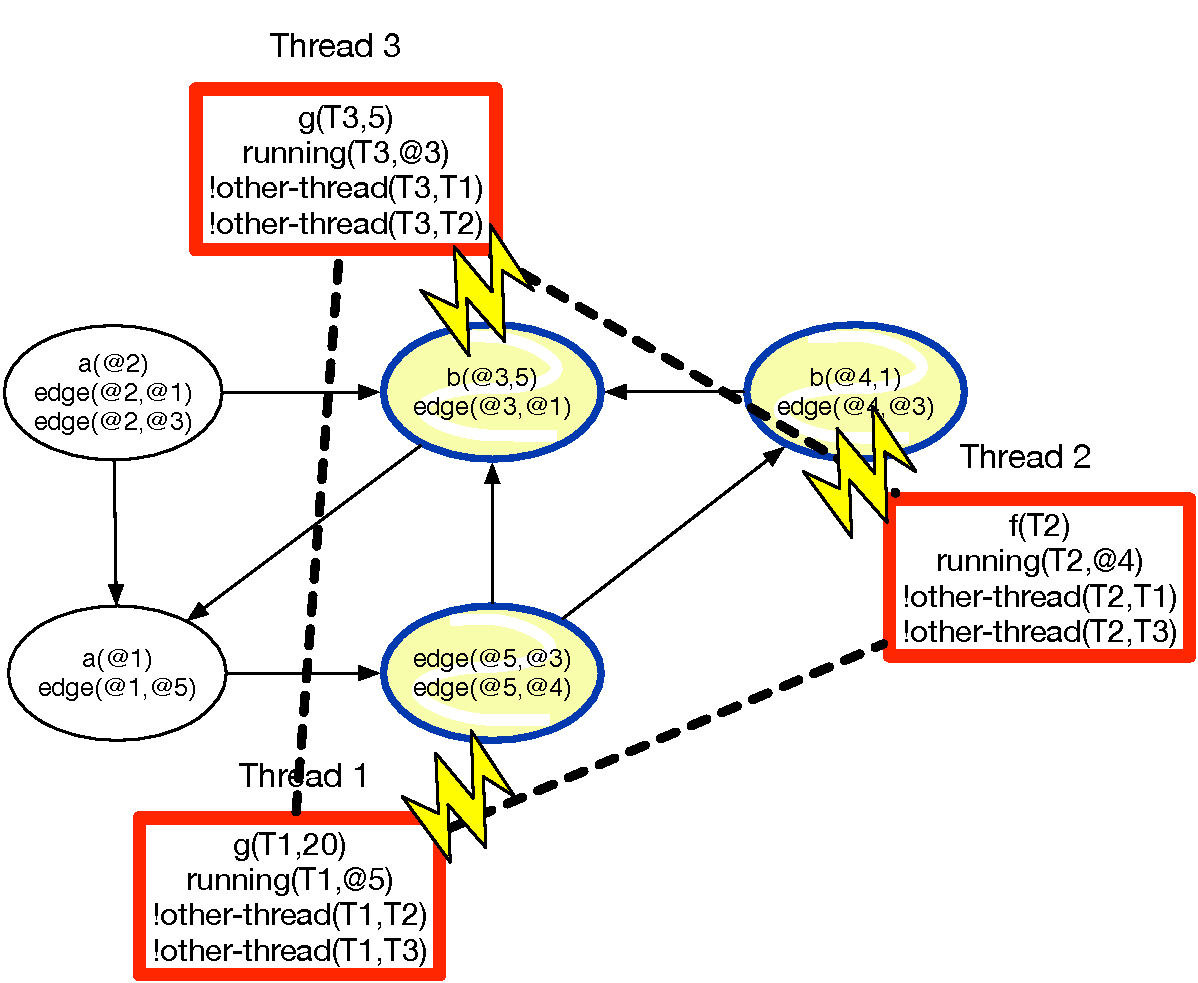
\includegraphics[width=0.6\linewidth]{figures/threads/threads.pdf}

   \caption{An example program being executed with three threads. Note that each
      threads has a \code{running} fact that stores the node currently being
   executed.}

   \label{fig:coord:thread_facts}
\end{figure}

We added several helpful predicates that allow the programmer to inspect the
graph of threads and reason about the state of computation as it relates to
threads:

\begin{itemize}
   \item \code{\bang thread-list(T, L)}: Fact instantiated in all threads where
      \code{L} is a list of all threads executing in the system.

   \item \code{\bang other-thread(T1, T2)}: Connects thread \code{T1} to all the
      other threads \code{T2} executing in the system. Note that in
      Fig.~\ref{fig:coord:thread_facts}, we use \code{\bang other-thread} fact
      to specify the graph of threads.


   \item \code{\bang leader-thread(T, TLeader)}: Fact instantiated in all
      threads where \code{TLeader} refers to a selected thread (the first thread
      in \code{L} of \code{\bang thread-list(T, L)}).

   \item \code{running(T, A)}: Used to retrieve the current node \code{A}
      running on thread \code{T}.
\end{itemize}

With the exception of \code{running}, every other fact is added at the beginning
of the program as a persistent fact.

\subsection{Reachability With Thread Facts}

We know update the graph reachability program presented in
Fig.~\ref{code:threads:reach_simple} to use thread facts in order to avoid
needless searches on the graph. The search process is still done concurrently as
before, but the search state is now stored in each thread, allowing the thread
to store partial results and coordinate with other threads. The code for this new
version is shown in Fig.~\ref{code:threads:reach_threads}.

Lines~\ref{line:threads:reacht_start1}-\ref{line:threads:reacht_start2} start
the search process by assigning a thread \code{Owner} to search \code{Id} using
the persistent fact \code{\bang thread-list} which contains the list of all
available threads in the system. Next, in
line~\ref{line:threads:reacht_threads}, a fact \code{thread-search} is created
for all threads using a comprehension. We use predicate \code{do-search} to
propagate the search through the graph and a predicate \code{visited} to mark
nodes already processed for a specific search.  The two rules in
lines~\ref{line:threads:reacht_check1}-\ref{line:threads:reacht_check2}
propagate the search process to the neighbor nodes and check if the current node
is part of the list of nodes we want to reach.

An interesting property of this version is that each owner thread responsible
for a search keeps track of the remaining nodes that need to be reached. In
line~\ref{line:threads:reacht_remove}, we derive \code{remove-thread-search} in
order to inform owner threads about new reachable nodes. Once an owner thread
detects that all nodes have been reached (lines
\ref{line:threads:reacht_reached1}-\ref{line:threads:reacht_reached2}), all the
other threads will know that and update their search state accordingly
(lines~\ref{line:threads:reacht_knows1}-\ref{line:threads:reacht_knows2}). When
every thread knows that all nodes were reached, they will consume
\code{do-search} facts (lines
\ref{line:threads:reacht_prune1}-\ref{line:threads:reacht_prune2}), effectively
pruning the search space.

\begin{figure}[h]
\begin{Verbatim}[numbers=left,fontsize=\codesize,commandchars=*\#\&]
search(A, Id, ToReach),*label#line:threads:reacht_start1&*hfill// Rule 1: initialize search
*textbf#!thread-list(T, L)&, Owner = nth(L, Id % @threads)*hfill// Allocate search to a thread
   -o {T2 | *textbf#!other-thread(T, T2)& -o *textbf#thread-search(T2, Id, ToReach, Owner)&},*label#line:threads:reacht_threads&
      do-search(A, Id).*label#line:threads:reacht_start2&

*textbf#thread-search(T, Id, [], Owner)&, *label#line:threads:reacht_prune1&*hfill// Rule 2: search completed
do-search(A, Id)
   -o *textbf#thread-search(T, Id, [], Owner)&. *label#line:threads:reacht_prune2&

do-search(A, Id),*hfill// Rule 3: node already visited
visited(A, Id)
   -o visited(A, Id).

do-search(A, Id),*label#line:threads:reacht_check1&*label#line:bfs_join1&*hfill// Rule 4: node found
*textbf#thread-search(T, Id, ToReach, Owner)&,*label#line:threads:reacht_join2&
!value(A, Val), Val in ToReach
   -o *textbf#thread-search(T, Id, remove(ToReach, Val), Owner)&,
      *textbf#remove-thread-search(Owner, Id, Val)&,*hfill// Tell owner thread about it.*label#line:threads:reacht_remove&
      {B | !edge(A, B) -o do-search(B, Id)},
      visited(A, Id).

do-search(A, Id),*hfill// Rule 5: node not found but propagate search
*textbf#thread-search(T, Id, ToReach, Owner)&,
!value(A, Val), ~ Val in ToReach
   -o *textbf#thread-search(T, Id, ToReach, Owner)&,
      visited(A, Id),
      {B | !edge(A, B) -o do-search(B, Id)}.*label#line:threads:reacht_check2&

*textbf#remove-thread-search(T, Id, Val), thread-search(T, Id, ToReach, Owner)&*hfill// Rule 6: node found
   *textbf#-o thread-search(T, Id, remove(ToReach, Val), Owner),&
      *textbf#check-results(T, Id).&

*textbf#check-results(T, Id),&*label#line:threads:reacht_reached1&*hfill// Rule 7: search is completed
*textbf#thread-search(T, Id, [], Owner)&
   *textbf#-o thread-search(A, Id, [], Owner),&
      *textbf#{B | !other-thread(T, B) -o signal-thread(B, Id)}.&*label#line:threads:reacht_reached2&

 *textbf#check-results(T, Id),&*hfill// Rule 8: search not completed yet
 *textbf#thread-search(T, Id, ToReach, Owner), ToReach <> []&
   *textbf#-o thread-search(T, Id, ToReach, Owner).&

*textbf#signal-thread(T, Id),&*hfill// Rule 9: thread knows search is done*label#line:threads:reacht_knows1&
*textbf#thread-search(T, Id, ToReach, Owner)&
   *textbf#-o thread-search(T, Id, [], Owner).& *label#line:threads:reacht_knows2&
\end{Verbatim}
\caption{Coordinated version of the reachability checking program. Note
that \code{@threads} represent the number of threads in the system.}
\label{code:threads:reach_threads}
\end{figure}

An alternative implementation could force every thread to share its reached
nodes to all the other threads in the system. However, this would generate a lot
of traffic between threads, which would actually make the program perform worse.
Our final solution is a good trade off since it only forces threads to
coordinate when pruning can actually happen.

Figure~\ref{fig:threads:results_search} presents experimental results of the
graph reachability program using 4 different datasets. Except for Random, all
the datasets were already used in the MSSD program and were presented before.
The Random dataset is a randomly generated graph with 50000 nodes and about a
million edges.  In the plots, we show the run time of the version without thread
facts (\textbf{Regular}) and the version using thread facts called
\textbf{Threads}. We also show the speedup of the \textbf{Threads} and
\textbf{Regular} versions against the \textbf{Regular} version with 1 thread.

Our results indicate that using thread facts produces a significant reduction in
run time. This is especially true in the case of datasets with large number of
edges, since less facts are produced and propagated in the graph when the
threads know that the search has been completed. The results also show that, in
the case of the Facebook dataset, in which the number of queries is the same as
the number of nodes, the use of thread facts does not produce great improvements
due to the costs of managing the reachability results on each thread's database.
These costs are related to the need to index and lookup \code{thread-search}
facts on the \code{Id} argument every time a node is inspected.

\begin{figure}[]
        \centering
        \begin{subfigure}[b]{\plotsize\textwidth}
           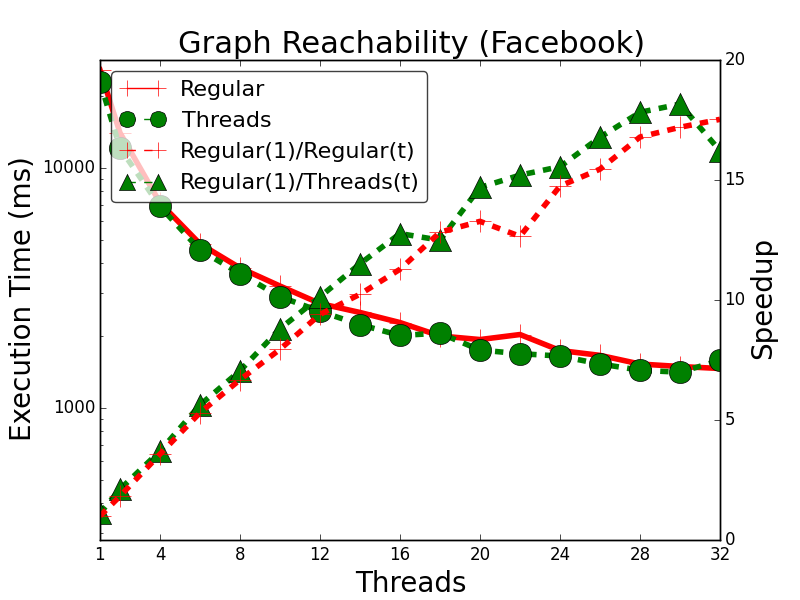
\includegraphics[width=\textwidth]{experiments/threads/cmp-search-facebook.png}
           \caption{Facebook has 2000 nodes and 20000 edges. The dataset makes
           2000 graph queries to 5\% of the graph's nodes.}
           \label{fig:threads:search_facebook}
        \end{subfigure}
        \spacing
        \begin{subfigure}[b]{\plotsize\textwidth}
           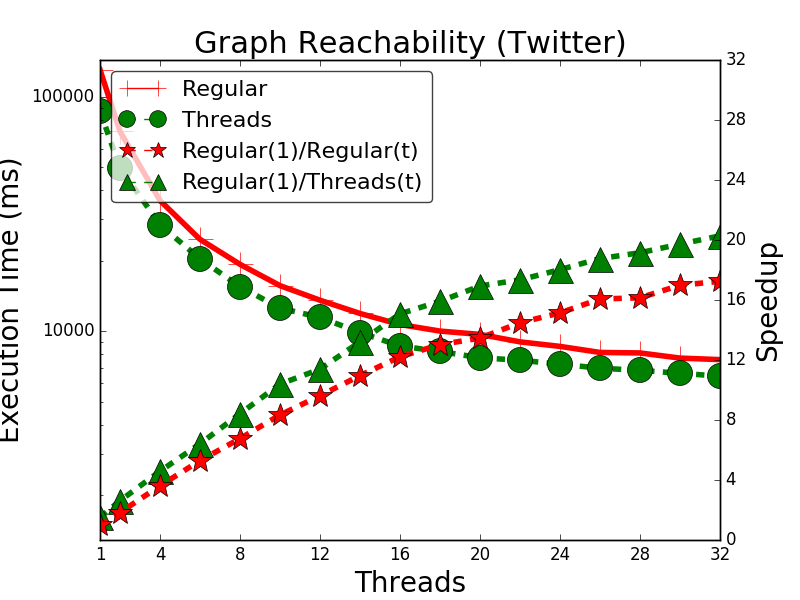
\includegraphics[width=\textwidth]{experiments/threads/cmp-search-twitter.png}
           \caption{Twitter has 81306 nodes and 1768149 edges. The dataset makes
           100 graph queries to 1\% of the graph's nodes.}
           \label{fig:threads:search_twitter}
        \end{subfigure} \\
        \begin{subfigure}[b]{\plotsize\textwidth}
           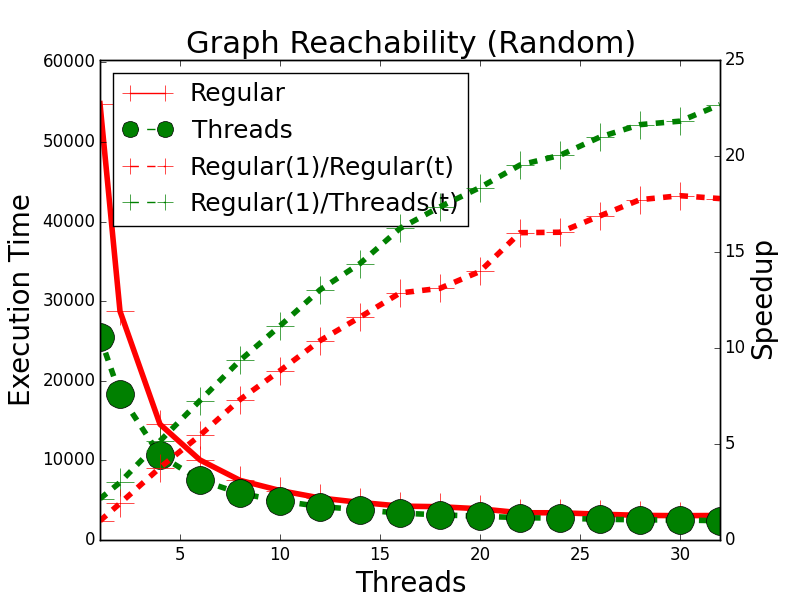
\includegraphics[width=\textwidth]{experiments/threads/cmp-search-random.png}
           \caption{Random is a graph with 50000 nodes and 1052674
              edges. The dataset makes 20 graph queries
              to 5\% of the graph's nodes.}
           \label{fig:threads:search_random}
        \end{subfigure}
        \spacing
        \begin{subfigure}[b]{\plotsize\textwidth}
           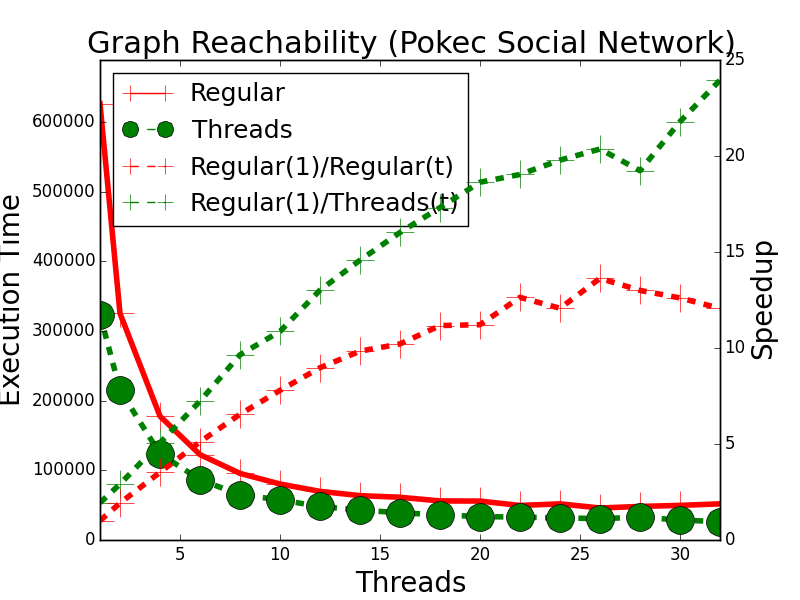
\includegraphics[width=\textwidth]{experiments/threads/cmp-search-pokec.png}
           \caption{Pokec has 1632803 nodes and 30622564 edges. The dataset
           makes 3 graph queries to 1\% of the graph's nodes.}
           \label{fig:threads:search_pokec}
        \end{subfigure} \\
        \caption{Measuring the performance of the graph reachability program
        when using thread facts.}
        \label{fig:threads:results_search}
\end{figure}

The graph reachability program shows how to introduce complex coordination
policies between threads by reasoning about the state of each thread. In
addition, the use of linear logic programming makes it easier to prove
properties of the program since computation is done by applying controlled
changes to the state.


\clearpage


\section{Implementation Changes}
The compilation and runtime system described in
Chapter~\ref{chapter:implementation} requires ysome changes in both the compiler
and in the runtime system to support thread-based facts.

\subsection{Compiler}

The compiler needs to recognize rules that use thread facts. For thread rules,
the compiler checks if the rule's body is using facts from the same thread by
checking the first argument of each fact. For mixed rules, the rule's body may
use a thread \code{T} and a node \code{A} and all the node facts have to use
\code{A}, while all threads facts must use \code{T} as the first argument. If
the programmer was to retrieve either the thread or the node for the current
computation, she may use \code{running(T, A)}.

Once rules are type checked, the iteration code for thread-based facts
needs to change. The database iterator will refer to the current thread in order to
fetch candidate facts since using the standard node database will return an
empty iterator. The runtime API used for inserting thread facts is also
different since they have to be added to the thread's database.

\subsection{Runtime}

Each thread has its own database of facts that is identical to a regular node
but only contains thread predicates. The major difference between a regular node
and a thread node is that a thread node is never put into the work queue of its
thread. As shown in the updated work loop presented in
Fig.~\ref{alg:threads:work_loop}, the thread node executes alongside the regular
node when $TH.process\_node$ is called. It is also important to note that,
before a thread becomes idle, it may have potential candidate thread rules that
are now derivable because another thread has derived thread facts in the current
thread. Note that it is entirely possible to have programs that only deal with
thread facts. These kinds of programs use only explicit parallelism.

\begin{figure}
\begin{algorithm}[H]
\KwData{Thread TH, THREADS}
\While{true}{
  $node \longleftarrow TH.work\_queue.pop\_node()$ \;
  \uIf{$node$}{
        \tcc{Have to use the thread's node}
        \underline{$TH.process\_node(node, TH.my\_node)$}\;
  }
  \Else{
     $target \longleftarrow random(len(THREADS))$\;
     $i \longleftarrow 0$\;
     \For{$i < len(THREADS)$}{
        $target \longleftarrow (target + 1) \% len(THREADS)$\;
        $nodes = THREADS[target].steal\_half()$\;
        \If{$len(nodes) > 0$}{                                                                                                    $TH.work\_queue.add\_to\_queue(nodes)$\;
           break\;
        }
        $i \longleftarrow i + 1$\;
     }
     \If{$len(TH.work\_queue) == 0$}{
        \tcc{The thread's node may have candidate rules using incoming thread facts}
        \underline{$TH.process\_node(nil, TH.my\_node)$}\;
        $TH.become\_idle()$\;
        \If{$TH.synchronize\_termination()$}{
           \Return{}\;
        }
        $TH.become\_active()$\;
     }
  }
}
\end{algorithm}
\caption{Thread work loop updated to take into account thread-based facts.
New and modified code is underlined.}
\label{alg:threads:work_loop}
\end{figure}

Thread facts also add points of synchronization the runtime system. For
instance, when a rule derives a new thread fact on another thread, it needs to
synchronize with that thread (using locks) to add the facts to the thread's
database.

\subsubsection{Matching Rules}

Matching rules using thread facts requires special care since some rules may
require both facts from a node and from a thread. Before a node is executed, the
matching engine of the regular node is updated to take into account the facts in
the thread. If the mixed rules are activated, they need to be executed, even if
they have failed under a different node. The reason is simple: the rule
constraints may now hold under the current node's database and therefore the
rule needs to be executed again.

\subsection{Graph Of Threads}

We added several helpful predicates that allow the programmer to inspect the
graph of threads and reason about the state of computation as it relates to
threads.

\begin{itemize}
   \item \code{\bang thread-list(T, L)}: Fact instantiated in all threads where
      \code{L} is a list of all threads executing in the system.

   \item \code{\bang other-thread(T1, T2)}: Connects thread \code{T1} to all the
      other threads \code{T2} executing in the system.

   \item \code{\bang leader-thread(T, TLeader)}: Fact instantiated in all
      threads where \code{TLeader} refers to a selected thread (usually the
      first thread in \code{L} of \code{\bang thread-list(T, L)}).

   \item \code{running(T, A)}: Used to retrieve the current node \code{A}
      running on thread \code{T}.
\end{itemize}

With the exception of \code{running}, every other fact is added at the beginning
of the program as a persistent axiom.


\section{Applications}

This section presents more applications that demonstrate the usefulness and
power of thread-based facts.

\subsection{Binary Search Trees: Caching Results}
In Section~\ref{sec:language:key_value} we have presented an algorithm for
replacing a key's value in a BST dictionary. To make the program more
interesting, we consider a sequence of $n$ lookup or replace operations for
different keys in the BST (which may or may not be repeated). A single lookup or
replace has worst-case time complexity $\mathcal{O}(h)$ where $h$ is the height
of the BST, therefore performing $n$ operations takes $\mathcal{O}(h \times n)$
time.

In order to reduce the execution time of the new program, we can cache the
search and replace operations so that repeated operations become faster. Instead
of traversing the entire height of the BST, we look in the cache and send the
operation immediately to the node where the key is located. Without thread
facts, we might have cached the results at the root node, however, this is not a
scalable approach as it would introduce a serious bottleneck.

Figure~\ref{code:threads:btree_lookup_cache} shows the updated BST code with a thread
cache. We just added two more predicates, \code{cache} and
\code{cache-size}, that are facts placed in the thread and represent cached
keys and the total size of the cache, respectively. We also added three new
rules that handle the following cases:

\begin{enumerate}
      \item A key is found and is also in the cache
         (lines~\ref{line:threads:kv_rule1_start}-\ref{line:threads:kv_rule2_end})

      \item A key is found but is not in the cache
         (lines~\ref{line:threads:kv_rule2_start}-\ref{line:threads:kv_rule2_end});

      \item A key is in the cache, therefore a \code{replace} fact is
         derived in the target node
         (lines~\ref{line:threads:kv_rule3_start}-\ref{line:threads:kv_rule3_end}).

\end{enumerate}

Note that it is quite easy to extend the cache mechanism to use an LRU type
approach in order to limit the size of the cache.

\begin{figure}[ht]
\begin{Verbatim}[numbers=left,fontsize=\codesize,commandchars=*\{\}]
type left(node, node).
type right(node, node).
type linear value(node, int Key, string Value).
type linear replace(node, int Key, string Value).
type linear cache(thread, node, int).
type linear cache-size(thread, int).

// (1) Key exists and is also in the cache.*label{line:threads:kv_rule1_start}
replace(A, Key, RValue),
value(A, Key, Value),
*textbf{cache(T, A, Key)}
   -o value(A, Key, RValue).
      *textbf{cache(T, A, Key)}.*label{line:threads:kv_rule1_end}

// (2) Key exists and is not in the cache.*label{line:threads:kv_rule2_start}
replace(A, Key, RValue),
value(A, Key, Value),
*textbf{cache-size(T, Total)}
   -o value(A, Key, RValue),
      *textbf{cache-size(T, Total + 1)},
      *textbf{cache(T, A, Key)}.*label{line:threads:kv_rule2_end}

// (3) Cached by the thread.*label{line:threads:kv_rule3_start}
replace(A, RKey, RValue),
*textbf{cache(T, TargetNode, RKey)}
   -o replace(TargetNode, RKey, RValue),
      *textbf{cache(T, TargetNode, RKey)}.*label{line:threads:kv_rule3_end}

replace(A, RKey, RValue),
value(A, Key, Value),
!left(A, B),
RKey < Key
   -o value(A, Key, Value),
      replace(B, RKey, RValue). // go left

replace(A, RKey, RValue),
value(A, Key, Value),
!right(A, B),
RKey > Key
   -o value(A, Key, Value),
      replace(B, RKey, RValue). // go right
\end{Verbatim}
\caption{LM program for performing lookups in a BST with a thread cache.}
\label{code:threads:btree_lookup_cache}
\end{figure}


\subsection{PowerGrid Problem}
Consider a power grid with $C$ consumers and $G$ generators. We are interested
in connecting each consumer to a single generator, but each generator has a
limited capacity and the consumer draws a certain amount of power from the
generator. A valid power grid is built in such a way that all consumers are
serviced by a generator and that no generator is being overdrawn by too many
consumers. Although consumers and generators may be connected through a complex
network, we analyze the simple case where any consumer is able to attach to any
generator.

\begin{wrapfigure}{r}{0.5\textwidth}
   \begin{center}
      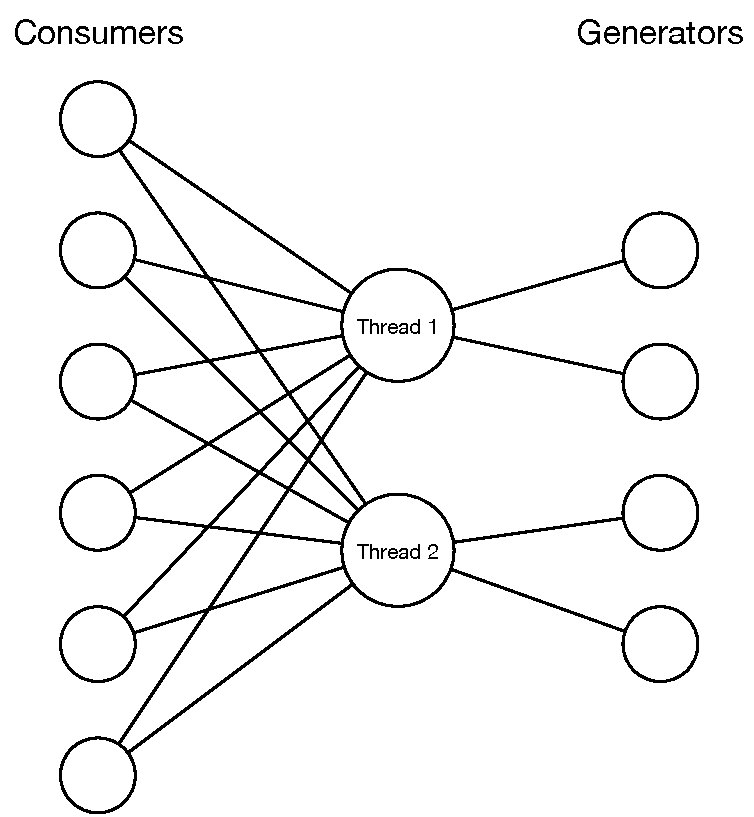
\includegraphics[width=1\linewidth]{figures/threads/powergrid.pdf}
   \end{center}
   \mycap{Configuration of a powergrid with 6 consumers, 4
      generators and 2 threads, with each thread responsible for 2 generators.}
   \label{fig:threads:powergrid}
\end{wrapfigure}

A straightforward distributed implementation for the PowerGrid problem requires
that each consumer is able to connect to any generator. Once a generator
receives a connection request, it may or may not accept it. If the generator has
no power available for the new consumer, it will disconnect from it and the
consumer must select another generator. This randomized algorithm works but may
take a long time to converge, depending on the amount of power available in the
generators. Figure~\ref{code:threads:powergrid} shows the LM code for this
solution. Consumer and generators node types are declared in
lines~\ref{line:threads:pg_decl1}-\ref{line:threads:pg_decl2} using the
\code{node} declaration, allowing us to have different predicates for consumers
and generators. The \code{consumer} and \code{generator} types become a subtype
of \emph{node}, that is, $consumer <: node$ and $generator <: node$.  These
subtypes allow us to declare initial facts that only apply to either the
\code{consumer} or \code{generator} subtype.

\begin{figure}[h!]
\begin{LineCode}[commandchars=*\#\&]
node generator.*label#line:threads:pg_decl1&*hfill// Type declaration
node consumer.*label#line:threads:pg_decl2&
type linear capacity(generator, int Total, int Used).*hfill// Predicate declaration
type linear connected-to(generator, consumer, int).
type linear connected-to-list(generator, list consumer).
type power(consumer, int).
type linear disconnected(consumer).
type linear connected(consumer, generator).
type generators(consumer, list generator).
type linear fails(generator, int).
type linear random-reconnect(generator).
type linear reconnect(consumer).
type linear connect(generator, consumer, int).
type linear disconnect(consumer, generator).

fails(G, Fails), Fails > maxfails*label#line:threads:pg_recon1&*hfill// Rule 1: disconnect one consumer
   -o random-reconnect(G).

capacity(G, Total, Used), random-reconnect(G),*hfill// Rule 2: disconnect one consumer
connected-to-list(G, L), L <> [], C = nth(L, randint(length(L))),
connected-to(G, C, Power)
   -o fails(G, 0), capacity(G, Total, Used - Power),
      connected-to-list(G, remove(L, C)), disconnect(C, G).

capacity(G, Total, Used), random-reconnect(G)*hfill// Rule 3: unable to disconnect one consumer
   -o capacity(G, Total, Used), fails(G, 0).*label#line:threads:pg_recon2&

connect(G, C, Power), capacity(G, Total, Used),*label#line:threads:pg_gen1&*hfill// Rule 4: connect consumer
fails(G, Fails), connected-to-list(G, L), Used + Power <= Total
   -o capacity(G, Total, Used + Power),
      fails(G, max(Fails - 1, 0)), connected-to(G, C, Power),
      connected-to-list(G, [C | L]).*label#line:threads:pg_gen2&

connect(G, C, Power), capacity(G, Total, Used),*label#line:threads:pg_fail1&*hfill// Rule 5: unable to connect consumer
Used + Power > Total, fails(G, Fails)
   -o capacity(G, Total, Used), disconnect(C, G),
      fails(G, Fails + 1).*label#line:threads:pg_fail2&

!generators(C, L), !power(C, Power),*label#line:threads:pg_connect1&*hfill// Rule 6: connect to a generator
reconnect(C), disconnected(C),
G = nth(L, randint(num-generators))
   -o connected(C, G), connect(G, C, Power).*label#line:threads:pg_connect2&

disconnect(C, G), connected(C, G)*hfill// Rule 7: finish disconnection
   -o disconnected(C), reconnect(C).

connected-to-list(G, []). fails(G, 0).*hfill// Initial facts
disconnected(C). reconnect(C). !generators(C, all-generators).
\end{LineCode}
\mycap{LM code for the regular PowerGrid program.}
\label{code:threads:powergrid}
\end{figure}

An example PowerGrid configuration with its initial facts is presented in
Fig.~\ref{code:threads:powergrid_init}. Consumers have a persistent fact
\code{!power(A, P)}, where \code{P} is the amount of power required by the
consumer. Consumers also start with a
\code{reconnect} fact that is used in
lines~\ref{line:threads:pg_connect1}-\ref{line:threads:pg_connect2} in order to
randomly select a generator from list \code{L} in the \code{!generators(A, L)}
fact. The generators have a \code{connect-to-list(A, L)} fact that manages the
list of connected consumers. The generator fact \code{capacity(A, Total, Used)},
stores the \code{Total} capacity of the generator and the amount of power
currently being \code{Used} (\code{Used < Total} at any point in the program).

Consumers and generators complete a connection when the generator receives a
\code{connect} fact which is used in
lines~\ref{line:threads:pg_gen1}-\ref{line:threads:pg_gen2} when the generator
has enough power for the new consumer. When there is not enough power
(\code{Used + Power > Total}), the generator disconnects the consumer in
lines~\ref{line:threads:pg_fail1}-\ref{line:threads:pg_fail2}. Note that each
generator maintains a \code{fail} fact that counts the number of times the
consumers have failed to connected. If there is too many failures, then the
generator decides to disconnect one consumer already connected in
lines~\ref{line:threads:pg_recon1}-\ref{line:threads:pg_recon2}, allowing for
different combinations to happen. In Fig.~\ref{code:threads:powergrid_final} we
present the final database of the example PowerGrid configuration, which shows
that all consumers have been able to find a suitable generator.

\begin{figure}[h!]
\begin{LineCode}[commandchars=*\#\&]
const generators = [@7, @8, @9, @10].

reconnect(@1).   !generators(@1, generators).   !power(@1, 5).
reconnect(@2).   !generators(@2, generators).   !power(@2, 10).
reconnect(@3).   !generators(@3, generators).   !power(@3, 5).
reconnect(@4).   !generators(@4, generators).   !power(@4, 10).
reconnect(@5).   !generators(@5, generators).   !power(@5, 10).
reconnect(@6).   !generators(@6, generators).   !power(@6, 5).

connected-to-list(@7, []).    capacity(@7, 15, 0).   fail(@7, 0).
connected-to-list(@8, []).    capacity(@8, 15, 0).   fail(@8, 0).
connected-to-list(@9, []).    capacity(@9, 10, 0).   fail(@9, 0).
connected-to-list(@10, []).   capacity(@10, 5, 0).   fail(@10, 0).
\end{LineCode}
\mycap{Initial facts for a PowerGrid configuration of 6 consumers and 4 generators.}
\label{code:threads:powergrid_init}
\end{figure}

\begin{figure}[h!]
\begin{LineCode}[commandchars=*\#\&]
connected(@1, @7).    !power(@1, 5).
connected(@2, @7).    !power(@2, 10).
connected(@3, @8).    !power(@3, 5).
connected(@4, @8).    !power(@4, 10).
connected(@5, @9).    !power(@5, 10).
connected(@6, @10).   !power(@6, 5).

connected-to-list(@7, [@1, @2]).   connected-to(@7, @1, 5).   connected-to(@7, @2, 10).
connected-to-list(@8, [@3, @4]).   connected-to(@8, @3, 5).   connected-to(@8, @4, 10).
connected-to-list(@9, [@5]).       connected-to(@9, @5, 10).
connected-to-list(@10, [@6]).      connected-to(@10, @6, 5).
capacity(@7, 15, 15).
capacity(@8, 15, 15).
capacity(@9, 10, 10).
capacity(@10, 5, 5).
\end{LineCode}
\mycap{Final facts for a PowerGrid configuration of 6 consumers and 4 generators.}
\label{code:threads:powergrid_final}
\end{figure}

The issue with this initial implementation presented in
Fig.~\ref{code:threads:powergrid} is that it lacks a global view of the problem,
which introduces inefficiencies and more communication between consumers and
generators. A better algorithm will require a more sophisticated communication
pattern between the nodes. As we have seen before, thread local facts are an
excellent mechanism to introduce a global view of the problem without
complicating the original algorithm written in a declarative style. For our
solution, we will partition the set of generators $G$ among the threads in the
system and make each thread assume the ownership of its generators. Each thread
can then process consumers with a global view over its set of generators,
allowing the immediate assignment of consumers to generators.
Figure~\ref{fig:threads:powergrid} shows how the configuration presented
previously is adjusted to take into account the number of available threads.

The LM code using thread facts shown in Fig.~\ref{code:threads:powergridt}. It uses
4 thread predicates: \code{thread-connected-to} and
\code{thread-connected-to-list} assign consumers to the generators owned by the
thread; \code{thread-capacity} stores the capacity of each generator assigned to
the thread; and \code{thread-total-capacity} provides a capacity overview of all
the generators owned by the thread.  The program starts with the rule in
lines~\ref{line:threads:pgt_start1}-\ref{line:threads:pgt_start2} by moving
generators to their corresponding threads using \code{set-thread}. Once the
generator is executing on the proper thread, the rule in
lines~\ref{line:threads:pgt_moved1}-\ref{line:threads:pgt_moved2} is derived
with the \code{just-moved} coordination fact and the state of the thread is
initialized. Consumers connect with the thread's generators with the rule in
lines~\ref{line:threads:pgt_con1}-\ref{line:threads:pgt_con2} by selecting the
first generator with enough power and then by updating the state of the thread.
Otherwise, if the thread does not have a suitable generator, a generator is
randomly selected using the method described before. For such cases, the thread
assigned with the selected generator will derive the rules in
lines~\ref{line:threads:pgt_gen1}-\ref{line:threads:pgt_gen2} and the thread
state is updated accordingly.

\begin{figure}[h!]
\begin{LineCode}[fontsize=\scriptsize,commandchars=*\#\&]
type linear thread-connected-to(thread, generator, consumer, int).*hfill// Predicate declaration
type linear thread-connected-to-list(thread, generator, list consumer).
type linear thread-capacity(thread, generator, int, int).
type linear thread-total-capacity(thread, int, int).
type linear start(generator).

start(G), !generator-id(G, Id)*label#line:threads:pgt_start1&
   -o set-thread(G, Id % @threads).*label#line:threads:pgt_start2&

just-moved(G), capacity(G, Total, Used), thread-total-capacity(T, TotalCapacity, TotalUsed)*label#line:threads:pgt_moved1&
   -o thread-connected-to-list(T, G, []), thread-capacity(T, G, Total, Used),
      thread-total-capacity(T, Total + TotalCapacity, Used + TotalUsed).*label#line:threads:pgt_moved2&

fails(G, Fails), Fails > maxfails
   -o random-reconnect(G).

thread-capacity(T, G, Total, Used), thread-total-capacity(T, TotalCapacity, TotalUsed),
random-reconnect(G), thread-connected-to-list(T, G, L), L <> [], C = nth(L, randint(length(L))),
thread-connected-to(T, G, C, Power), NewUsed = Used - Power
   -o fails(G, 0), thread-capacity(T, G, Total, NewUsed),
      thread-total-capacity(T, TotalCapacity, TotalUsed - Power),
      thread-connected-to-list(T, G, remove(L, C)), disconnect(C, G).

random-reconnect(G) -o fails(G, 0).

connect(G, C, Power), thread-total-capacity(T, TotalCapacity, TotalUsed),*label#line:threads:pgt_gen1&
thread-capacity(T, G, Total, Used), fails(G, Fails), thread-connected-to-list(T, G, L),
NewUsed = Used + Power, NewUsed <= Total
   -o thread-capacity(T, G, Total, NewUsed),
      thread-total-capacity(T, TotalCapacity, TotalUsed + Power),
      fails(G, max(Fails - 1, 0)), thread-connected-to(T, G, C, Power),
      thread-connected-to-list(T, G, [C | L]).*label#line:threads:pgt_gen11&

connect(G, C, Power), thread-capacity(T, G, Total, Used), Used + Power > Total, fails(G, Fails)
   -o thread-capacity(T, G, Total, Used), disconnect(C, G), fails(G, Fails + 1).*label#line:threads:pgt_gen2&

!power(C, Power), reconnect(C), disconnected(C), thread-total-capacity(T, TotalCapacity, TotalUsed),*label#line:threads:pgt_con1&
TotalNewUsed = TotalUsed + Power, NewUsed <= TotalCapacity,
thread-capacity(T, G, Total, Used), thread-connected-to-list(T, G, ConnectList),
NewUsed = Used + Power, NewUsed <= Total
   -o connected(C, G), thread-capacity(T, G, Total, NewUsed),
      thread-connected-to-list(T, G, [C | ConnectList]), thread-connected-to(T, G, C, Power),
      thread-total-capacity(T, TotalCapacity, TotalNewUsed).*label#line:threads:pgt_con2&

!generators(C, L), !power(C, Power), reconnect(C), disconnected(C), G = nth(L, randint(num-generators))*label#line:threads:pgt_conn1&
   -o connected(C, G), connect(G, C, Power).*label#line:threads:pgt_conn2&

disconnect(C, G), connected(C, G)
   -o disconnected(C), reconnect(C).

thread-total-capacity(T, 0, 0).*hfill// Initial facts
fails(G, 0).  disconnected(C).  reconnect(C).  !generators(C, all-generators).  start(G).
\end{LineCode}
\mycap{LM code for the optimized PowerGrid program.}
\label{code:threads:powergridt}
\end{figure}

The experimental results for the PowerGrid program are presented in
Fig.~\ref{fig:threads:results_powergrid}. In the plots, we show the run time of
the version without thread facts, named \textbf{Regular}, and the version using
thread facts, called \textbf{Threads}. We also show the speedup of the
\textbf{Threads} and \textbf{Regular} versions against the \textbf{Regular}
version with 1 thread.  We experimented with four datasets:

\begin{enumerate}
      \item 0.5 M C / 2000 G: Half a million consumers connected to 2000
         generators. This is the baseline dataset.

      \item 0.5 M C / 64 G: Half a million consumers connected to 64
         generators. This is similar to the previous dataset, but the number of
         generators is much smaller.

      \item 1 M C / 4000 G / Low Variability: 1 million consumers connected to
         4000 generators. The capacity of each generator has low variability so
         that each generator has a similar capacity.

      \item 1 M C / 4000 G / High Variability: 1 million consumers connected to
         4000 generators. The capacity of each generator has high variability so
         that some generators have no capacity or three times the average the
         capacity.

\end{enumerate}

All the datasets were generated randomly so that the total capacity of the
generators is about 2\% more than the required consumer capacity. The capacity
of each generator is generated randomly and, except for the last two datasets,
the capacity is between 0 and twice the average capacity (total capacity divided
by the number of generators).

The first important observation relates to the first two datasets. In the 0.5 M
C / 2000 G, the \textbf{Threads} version has more than a 150-fold speedup for 32
threads while the 0.5 M C / 64 G dataset only reaches a 70-fold speedup. Having
only 64 generators instead of 2000 makes it harder to scale the program since
there is only a few generators to distribute among threads. However, it must be
noted that the 0.5 M C / 64 G dataset performs proportionally faster when using
1 thread than the 2000 G dataset since that one thread has a small number of
generators to choose from when processing consumers. The rule that assigns
generators to consumers
(lines~\ref{line:threads:pgt_gen1}-\ref{line:threads:pgt_gen11} in
Fig.~\ref{code:threads:powergridt}) needs to
iterate through all the generators to find one with enough power to handle the
consumer, therefore, a smaller number of generators is a clear advantage over
having many generators in the case of using just 1 thread.

\begin{figure}[]
        \centering
        \begin{subfigure}[b]{\plotsize\textwidth}
           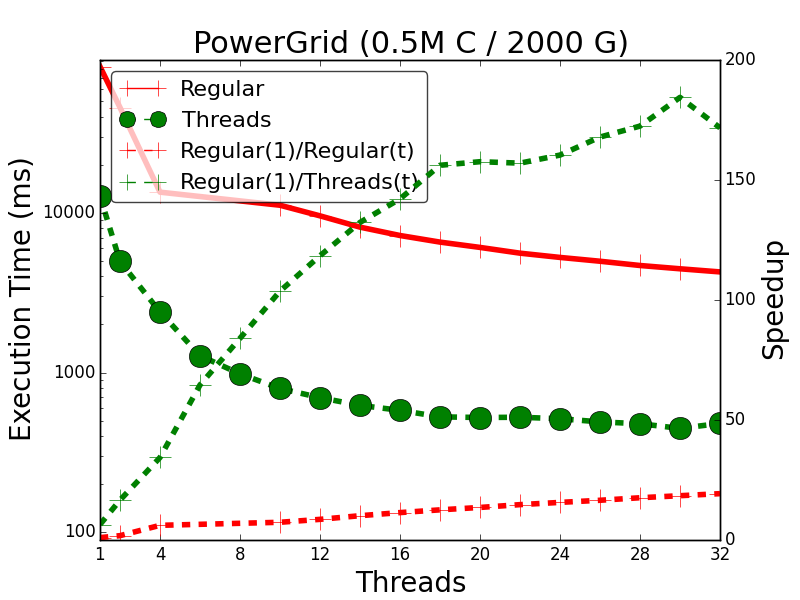
\includegraphics[width=\textwidth]{experiments/threads/cmp-powergrid-500000C2000G.png}
           \mycap{}
           \label{fig:threads:powergrid1}
        \end{subfigure}
        ~
        \begin{subfigure}[b]{\plotsize\textwidth}
           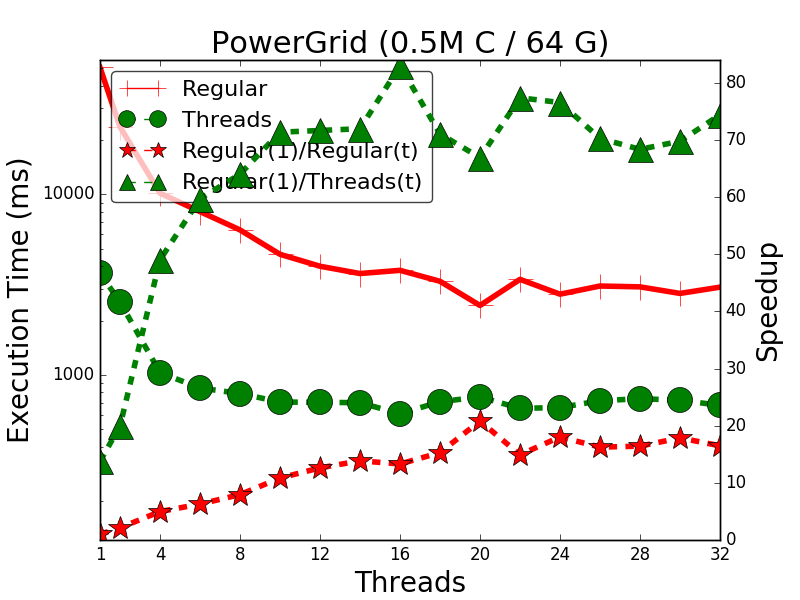
\includegraphics[width=\textwidth]{experiments/threads/cmp-powergrid-500000C64G.png}
           \mycap{}
           \label{fig:threads:powergrid2}
        \end{subfigure} \\
        \begin{subfigure}[b]{\plotsize\textwidth}
           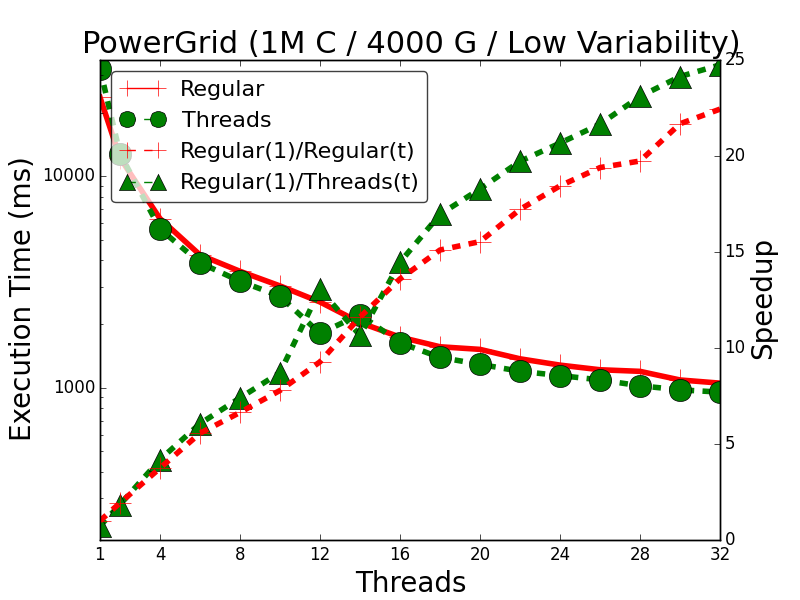
\includegraphics[width=\textwidth]{experiments/threads/cmp-powergrid-1M4000C-low.png}
           \mycap{}
           \label{fig:threads:powergrid3}
        \end{subfigure} ~
        \begin{subfigure}[b]{\plotsize\textwidth}
           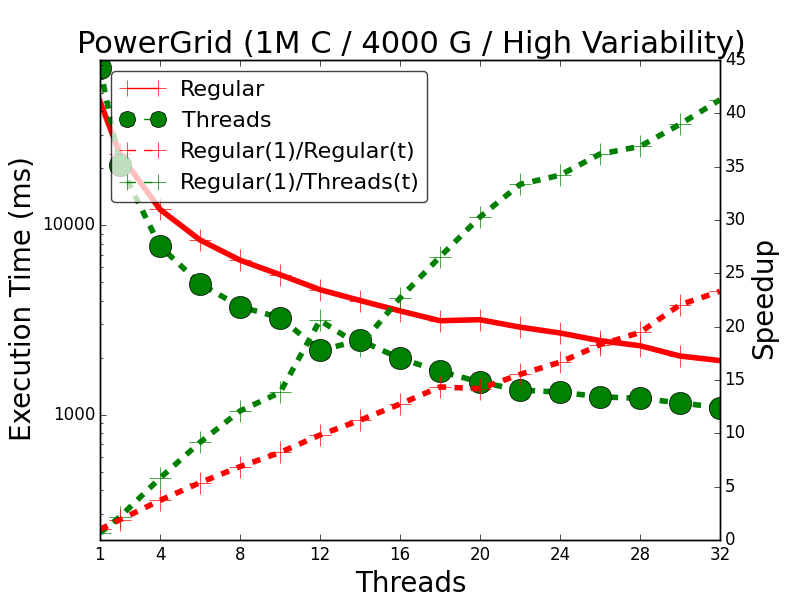
\includegraphics[width=\textwidth]{experiments/threads/cmp-powergrid-1M4000C-high.png}
           \mycap{}
           \label{fig:threads:powergrid4}
        \end{subfigure} \\
        \mycap{Measuring the performance of the PowerGrid program
        when using thread facts.}
        \label{fig:threads:results_powergrid}
\end{figure}

The second important observation relates to the last two datasets where we
experimented with a variable capacity for the generators. For the Low
Variability dataset, the consumers have identical capacities, while in the High
Variability dataset, generators have a more variable capacity, which should make
it harder for the algorithm to find a valid generator/consumer assignment.  Our
results show exactly that: the Low Variability shows a small difference between
the \textbf{Regular} and \textbf{Threads} version, while in the High Variability
dataset, the \textbf{Threads} version is much faster than the \textbf{Regular}
version. However, for the High Variability dataset, we were expecting a speedup
that was closer to the 0.5 M C / 2000 G dataset, since the number of generators
is much higher. Furthermore, if we compare the run times of the \textbf{Regular}
and \textbf{Threads} version when using 1 thread, we notice that the
\textbf{Threads} version is actually slower. As noted before, this may be due to
the fact that the LM rule for assigning generators to consumers needs to perform
a linear scan on the available generators to find a suitable generator which
then negatively impacts performance. This is a clear drawback of the logic
programming model that could potentially be solved by maintaining a sorted list
of \texttt{thread-capacity} facts.

In Table~\ref{table:threads:powergrid_stats}, we present several fact statistics
that compare the \textbf{Regular} version with the \textbf{Threads} version when
executing with multiple threads. The \textbf{\# Derived} column indicates the
number of derived facts, \textbf{\# Deleted} indicates the number of retracted
facts, while \textbf{\# Final} is the number of facts in the database after the
program terminates. The table results clearly show that using thread-based facts
results in a decrease in the number of generated facts, which is more
significant in the 0.5M C / 2000 G dataset (10-fold reduction). The table also
explains why this dataset performs much better than the 1M C / 4000 G High
Variability dataset, which only sees a 2-fold reduction in derived facts.

When comparing the number of facts derived when using a different number of
threads, the overall trend indicates that having more threads slightly increases
the number of derived facts. This is especially true for the 0.5 M C / 64 G
datasets, where twice as many facts are generated when using 32 threads when
compared to 1 thread.

\begin{table}[ht]
   \begin{center}
      \begin{tabular}{c | c || c c | c c | c c} \hline
	 \multirow{2}{*}{\textbf{Dataset}} & \multirow{2}{*}{\textbf{Threads}} & \multicolumn{2}{c|}{\textbf{\# Derived}} & \multicolumn{2}{c|}{\textbf{\# Deleted}} & \multicolumn{2}{c}{\textbf{\# Final}}\\
	 & & Regular & Threads & Regular & Threads & Regular & Threads\\ \hline \hline
\multirow{7}{*}{0.5M C / 2000 G}  & 1 &  49.7M & 4.2M &  48.2M & 2.5M &  2.5M & 2.5M \\
 & 2 &  48.5M & 4.4M &  47.7M & 2.5M &  2.5M & 2.5M \\
 & 4 &  49.4M & 4.1M &  47.9M & 2.6M &  2.5M & 2.5M \\
 & 8 &  49.4M & 4.10M &  47.9M & 2.5M &  2.5M & 2.5M \\
 & 16 &  50.8M & 4.1M &  49.3M & 2.6M &  2.5M & 2.5M \\
 & 24 &  49.8M & 4.2M &  48.3M & 2.7M &  2.5M & 2.5M \\
 & 32 &  49.3M & 4.6M &  47.8M & 3.1M &  2.5M & 2.5M \\
	\hline
\multirow{7}{*}{0.5M C / 64 G}  & 1 &  20.2M & 4.3M &  18.5M & 2.5M &  2.5M & 2.5M \\
 & 2 &  19.9M & 4.2M &  18.4M & 2.7M &  2.5M & 2.5M \\
 & 4 &  20.7M & 4.4M &  18.5M & 2.9M &  2.5M & 2.5M \\
 & 8 &  19.9M & 5.6M &  18.4M & 4.10M &  2.5M & 2.5M \\
 & 16 &  19.8M & 6.8M &  18.3M & 5.3M &  2.5M & 2.5M \\
 & 24 &  19.7M & 8.4M &  18.2M & 6.9M &  2.5M & 2.5M \\
 & 32 &  19.9M & 9.3M &  18.4M & 7.5M &  2.5M & 2.5M \\
	\hline
\multirow{7}{*}{\makecell{1M C / 4000 G \\Low Variability}}  & 1 &  9.4M & 7.5M &  6.4M & 4.5M &  5.1M & 5.1M \\
 & 2 &  9.4M & 7.5M &  6.4M & 4.5M &  5.1M & 5.1M \\
 & 4 &  9.4M & 7.5M &  6.4M & 4.5M &  5.1M & 5.1M \\
 & 8 &  9.4M & 7.6M &  6.4M & 4.6M &  5.1M & 5.1M \\
 & 16 &  9.4M & 7.5M &  6.4M & 4.5M &  5.1M & 5.1M \\
 & 24 &  9.4M & 7.6M &  6.3M & 4.6M &  5.1M & 5.1M \\
 & 32 &  9.3M & 7.5M &  6.3M & 4.5M &  5.1M & 5.1M \\
	\hline
\multirow{7}{*}{\makecell{1M C / 4000 G \\High Variability}}  & 1 &  16.4M & 8.8M &  13.4M & 5.8M &  5.1M & 5.1M \\
 & 2 &  16.5M & 8.8M &  13.5M & 5.8M &  5.1M & 5.1M \\
 & 4 &  16.5M & 8.8M &  13.4M & 5.8M &  5.1M & 5.1M \\
 & 8 &  16.5M & 8.9M &  13.5M & 5.9M &  5.1M & 5.1M \\
 & 16 &  16.5M & 8.8M &  13.5M & 5.8M &  5.1M & 5.1M \\
 & 24 &  16.5M & 9.3M &  13.5M & 6.2M &  5.1M & 5.1M \\
 & 32 &  16.5M & 9.6M &  13.5M & 6.5M &  5.1M & 5.1M \\
	\hline
\end{tabular}

   \end{center}

   \mycap{Measuring the reduction in derived facts when using thread-based
   facts.}
   \label{table:threads:powergrid_stats}
\end{table}

%\clearpage


\subsection{Splash Belief Propagation}\label{sec:coordination:bp}
Approximation algorithms can obtain significant benefits from using customized
scheduling policies since they follow important statistical properties and thus
can trade correctness for faster convergence. An example of such algorithm is
the Loopy Belief Propagation (LBP)~\cite{Murphy99loopybelief}. LBP is an
approximate inference algorithm used in graphical models with cycles which
employs a sum-product message passing algorithm where nodes exchange messages
with their immediate neighbors and apply some computations to the messages
received.

\begin{figure}[h]
   \begin{center}
      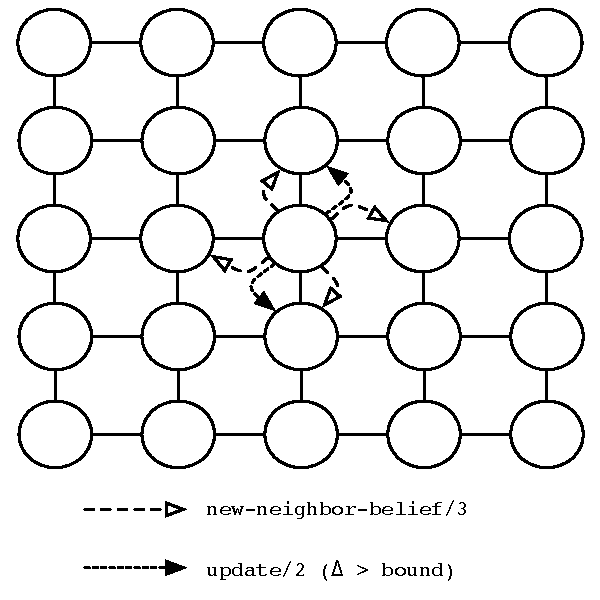
\includegraphics[width=0.3\textwidth]{figures/bp/bp.pdf}
   \end{center}

   \mycap{LBP communication patterns. \code{new-neighbor-belief} facts are
   sent to the neighborhood when the node's belief value is updated. If the new
   value sent to the neighbor differs significantly from the value sent before
   the current the round, then an \code{update} fact is also sent (to the node
   above and below in this case).}

\label{fig:coordination:bp}
\end{figure}

LBP is an algorithm that maps very well to the graph-based model of LM. The
original algorithm computes the belief of all nodes using several iterations
with synchronization between iterations. However, it is possible to avoid the
synchronization step, if we take advantage of the fact that LBP will converge
even when using an asynchronous approach. So, instead of computing the belief
iteratively, we keep track of all messages sent/received (and overwrite them
when we receive a new one) and recompute the belief asynchronously.
Figure~\ref{fig:coordination:bp} presents the communication patterns of the
program, while Fig.~\ref{code:coordination:bp} presents the LM code for the
asynchronous version of LBP.

\begin{figure}[ht]
\begin{Verbatim}[numbers=left, fontsize=\codesize, commandchars=\*\#\&]
type list float belief.*hfill// Type declaration.

type potential(node, belief).*hfill// Predicate declaration
type edge(node, node).
type linear neighbor-belief(node, node, belief).
type linear new-neighbor-belief(node, node, belief).
type linear sent-neighbor-belief(node, node, belief).
type linear check-residual(node, float, node).
type linear belief(node, belief).
type linear update-messages(node, belief).
type linear update(node).

neighbor-belief(A, B, Belief),*label#line:coord:bp_first1&*hfill// Rule 1: update neighbor belief value
new-neighbor-belief(A, B, NewBelief)
   -o neighbor-belief(A, B, NewBelief).*label#line:coord:bp_first2&

check-residual(A, Residual, B),*label#line:coord:bp_check1&*hfill// Rule 2: check residual
Residual > bound
   -o update(B).

check-residual(A, _, _) -o 1.*label#line:coord:bp_check2&*hfill// Rule 3: check residual

update-messages(A, NewBelief),*hfill// Rule 4: compute belief to be sent to a neighbor node*label#line:coord:bp_iterate1&
   -o {B, OldIn, OldOut, Cavity, Convolved, OutMessage, Residual |
         !edge(A, B),
         neighbor-belief(A, B, OldIn),
         sent-neighbor-belief(A, B, OldOut),
         Cavity = normalize(divide(NewBelief, OldIn)),
         Convolved = normalize(convolve(global-potential, Cavity)),
         OutMessage = damp(Convolved, OldOut, damping)
         Residual = residual(OutMessage, OldOut)
         -o check-residual(A, Residual, B),
            new-neighbor-belief(B, A, OutMessage),
            neighbor-belief(A, B, OldIn),
            sent-neighbor-belief(A, B, OutMessage)}.*label#line:coord:bp_iterate2&

*label#line:coord:bp_last1&
update(A), update(A) -o update(A).*label#line:coord:bp_update&*hfill// Rule 5: prune redundant update operations

update(A),*hfill// Rule 6: initiate update operation*label#line:coord:bp_update1&
!potential(A, Potential),
belief(A, MyBelief)
   -o [sum Potential => Belief; B, Belief |*label#line:coord:bp_agg1&
         neighbor-belief(A, B, Belief) -o
         neighbor-belief(A, B, Belief) ->
         Normalized = normalizestruct(Belief),
         update-messages(A, Normalized), belief(A, Normalized)].*label#line:coord:bp_last2&*label#line:coord:bp_update2&*label#line:coord:bp_agg2&
\end{Verbatim}

\mycap{LM code for the asynchronous version of the Loopy Belief Propagation
problem.}

\label{code:coordination:bp}
\end{figure}

\clearpage

Belief values are arrays of floats and are represented by \code{belief/2} facts.
The first rule (lines~\ref{line:coord:bp_first1}-\ref{line:coord:bp_first2})
updates a given neighbor belief whenever a new belief value is received. This is
the highest priority rule since we want to update the neighbor beliefs before
doing anything else. In order to store the belief values of the neighbor nodes,
we use \code{neighbor-belief/3} facts, where the second argument is the neighbor
address and the third argument is the belief value.

The last two rules (lines~\ref{line:coord:bp_last1}-\ref{line:coord:bp_last2})
update the belief value of a node. An \code{update} fact starts the process.
The first rule (line~\ref{line:coord:bp_update}) simply removes redundant
\code{update} facts and the second rule
(lines~\ref{line:coord:bp_update1}-\ref{line:coord:bp_update2}) performs the
belief update by aggregating all the neighbor belief values. The aggregate in
lines~\ref{line:coord:bp_agg1}-\ref{line:coord:bp_agg2} also derives copies of
the neighbors beliefs that need to be consumed in order to compute the belief
value that is going to be sent to the target neighbor. The aggregate uses a
custom accumulator that takes two arrays and adds the floating point numbers at
each index of the array.

The rule in lines~\ref{line:coord:bp_iterate1}-\ref{line:coord:bp_iterate2}
iterates through the neighbor belief values and sends new belief values by
performing the appropriate computations on the new belief value of the current
node and on the belief value sent previously. For each neighbor update, we also
check in lines~\ref{line:coord:bp_check1}-\ref{line:coord:bp_check2} if the
change in belief values is greater than \code{bound} (a program constant) and
then force the neighbor nodes to update their belief values by deriving
\code{update(B)}. This allows neighbor nodes to use updated neighbor values and
recompute their own belief values using more up-to-date information. The
computation of belief values will then start to converge to their true belief
values, independently of the node scheduling used.

However, if we prioritize nodes that receive new neighbor belief values with a
larger \code{Residual} then we may converge faster.
Figure~\ref{code:coordination:improved_bp} shows the fourth rule modified with a
\code{add-priority} fact, which increases the priority of neighbor nodes when
the source node has large changes in its belief value.

\begin{figure}[h!]
\begin{Verbatim}[numbers=left,commandchars=\\\{\},fontsize=\codesize]
update-messages(A, NewBelief),*hfill// Rule 4: compute belief to be sent to a neighbor node
   -o \{B, OldIn, OldOut, Cavity, Convolved, OutMessage, Residual |
         !edge(A, B),
         neighbor-belief(A, B, OldIn),
         sent-neighbor-belief(A, B, OldOut),
         Cavity = normalize(divide(NewBelief, OldIn)),
         Convolved = normalize(convolve(global-potential, Cavity)),
         OutMessage = damp(Convolved, OldOut, damping)
         Residual = residual(OutMessage, OldOut)
         -o check-residual(A, Residual, B),
            new-neighbor-belief(B, A, OutMessage),
            neighbor-belief(A, B, OldIn),
            \underline{add-priority(B, Residual)},
            sent-neighbor-belief(A, B, OutMessage)\}.
\end{Verbatim}
\mycap{Extending the LBP program with priorities.}
\label{code:coordination:improved_bp}
\end{figure}


The proposed asynchronous approach has shown to be an improvement over the
synchronous version because it leads to faster convergence time. An improved
evaluation strategy is the Splash Belief
Propagation~(SBP)~\cite{Gonzalez+al:aistats09paraml}, where belief values are
computed asynchronously by first building a tree and then updating the beliefs
of each node twice, first from the leaves to the root and then from the root to
the leaves These \emph{splash trees} are built by starting at a node whose
belief changed the most in the last update. The trees must be built iteratively
until convergence is achieved.

In an environment with $T$ threads, it is then possible to build $T$ splash
trees concurrently. First, we partition the nodes into $T$ regions and then
assign each region to a thread. A thread is then responsible for iteratively
building splash trees on that region until convergence is reached.
Fig.~\ref{fig:threads:splash_bp} shows a grid of nodes that has been partitioned
in two regions where splash trees will be built. To build a splash tree, a
thread starts from the highest priority node (the tree's root) from its region
and then performs a breadth-first search from that node to construct the rest of
the tree. The belief values are then computed in order.

\begin{figure}[ht]
   \begin{center}
      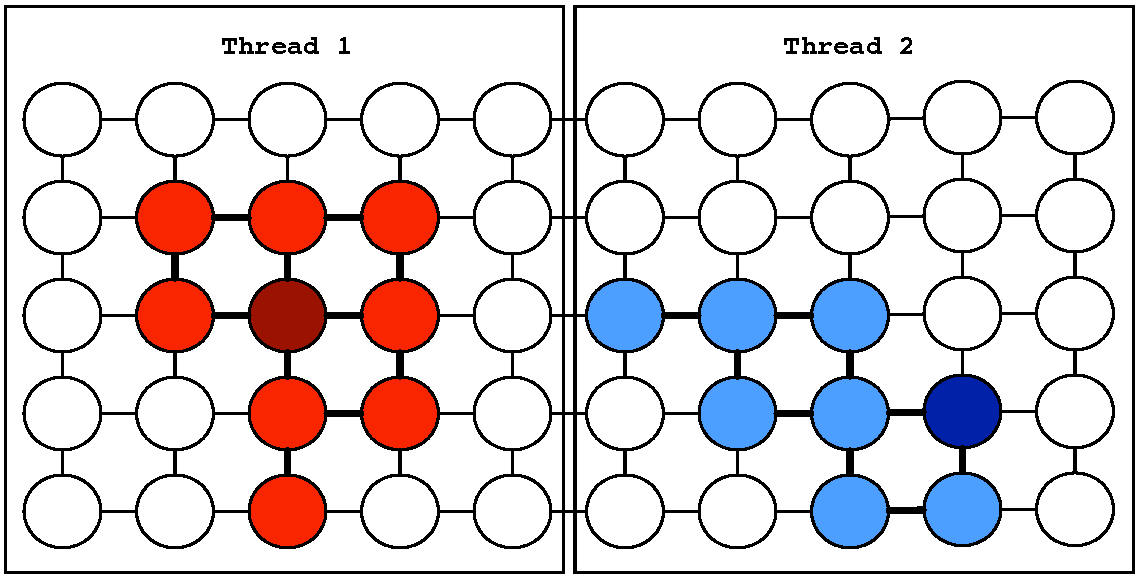
\includegraphics[width=0.7\linewidth]{figures/threads/splash_bp}
   \end{center}
   \caption{Creating splash trees using two threads. The graph is
      partitioned into two regions and each thread is able to build separate
   splash trees starting from the highest priority node.}
   \label{fig:threads:splash_bp}
\end{figure}

The LM implementation for SBP is shown in Fig.~\ref{code:threads:sbp}. First,
in lines \ref{line:threads:splash_part1}-\ref{line:threads:splash_part2}, we
partition the nodes into regions using \code{set-thread} and then we start the
creation of the first splash tree (line~\ref{line:threads:splash_first}) by
deriving \code{start-tree(T)}.  The remaining phases of the algorithm are
explained next.

\begin{figure}[!htb]
\begin{Verbatim}[numbers=left,commandchars=*\{\},fontsize=\codesize]
type list node tree.

type linear partitioning(thread, int). // Number of nodes to receive.
type linear start-tree(thread).
type linear new-tree(thread, tree, tree).
type linear expand-tree(thread, tree).
type linear first-phase(thread, tree, tree).
type linear second-phase(thread, tree).
type linear start(node).

start(A).
partitioning(T, @world / @threads). // Move @world/@threads nodes.

!coord(A, X, Y), start(A) // Moving this node.*label{line:threads:splash_part1}
   -o set-static(A), set-thread(A, grid(X, Y)).
just-moved(A), partitioning(T, Left) // Thread received another node.
   -o partitioning(T, Left - 1).
partitioning(T, 0) -o start-tree(T).*label{line:threads:splash_part2}*label{line:threads:splash_first}

start-tree(T),*label{line:threads:splash_building1} priority(A, P), P > 0.0 *hfill{} // Tree building
   -o priority(A, P), expand-tree(T, [A], []).*label{line:threads:splash_building2}
expand-tree(T, [A | All], Next)
   -o thread-id(A, Id),
      [collect => L ; | !edge(A, L), ~ L in All, ~ L in Next,*label{line:threads:splash_agg1} priority(L, P), P > 0.0,
         thread-id(L, Id2), Id1 = Id2 -o priority(L, P), thread-id(L, Id2) ->
         new-tree(T, [A | All],
            if len(All) + 1 >= maxnodes then [] else Next ++ L end)].*label{line:threads:splash_agg2}*label{line:threads:splash_next}

new-tree(T, [A | All], [])
   -o schedule-next(A), first-phase(T, reverse([A | All]), [A | All]).*label{line:threads:splash_first_phase}
new-tree(T, All, [B | Next])
   -o schedule-next(B), expand-tree(T, [B | All], Next).

first-phase(T, [A], [A]), running(T, A) *hfill{} // First phase
   -o running(T, A), update(A), remove-priority(A), start-tree(T).
first-phase(T, [A, B | Next], [A]), running(T, A)
   -o running(T, A), update(A), schedule-next(B), second-phase(T, [B | Next]).*label{line:threads:splash_first_update1}
first-phase(T, All, [A, B | Next]), running(T, A)
   -o running(T, A), update(A), schedule-next(B), first-phase(T, All, [B | Next]).*label{line:threads:splash_first_update2}

second-phase(T, [A]), running(T, A) *hfill{} // Second phase
   -o running(T, A), update(A), remove-priority(A), start-tree(T).*label{line:threads:splash_second_update1}
second-phase(T, [A, B | Next]), running(T, A)
   -o running(T, A), update(A), schedule-next(B), second-phase(T, [B | Next]).*label{line:threads:splash_second_update2}
\end{Verbatim}

   \caption{LM code for the Splash Belief Propagation program.}
  \label{code:threads:sbp}
\end{figure}

\begin{description}

   \item[Tree building:] Starts after the rule in lines
      \ref{line:threads:splash_building1}-\ref{line:threads:splash_building2} is
      derived. Since the thread always picks the highest priority node, we start
      by adding that node to the list that represents the tree. In lines
      \ref{line:threads:splash_agg1}-\ref{line:threads:splash_agg2}, we use an
      aggregate to gather all the neighbor nodes that have a positive priority
      (due to a new belief update) and are in the same thread. Nodes are
      collected into list \code{L} and appended to list \code{Next}
      (line~\ref{line:threads:splash_next}).

   \item[First phase:] When the number of nodes in the tree reaches a certain
      limit, a \code{first-phase} is generated to update the beliefs of all
      nodes in the tree (line~\ref{line:threads:splash_first_phase}). As the
      nodes are updated, starting from the leaves and ending at the root, an
      \code{update} fact is derived to update the belief values
      (lines~\ref{line:threads:splash_first_update1}
      and~\ref{line:threads:splash_first_update2}).

   \item[Second phase:] Performs the computation of beliefs from the root to the
      leaves and the belief values are updated a second time
      (lines~\ref{line:threads:splash_second_update1}
      and~\ref{line:threads:splash_second_update2}).

\end{description}

SBP is also implemented in GraphLab~\cite{GraphLab2010}, a C++ framework for
writing machine learning algorithms. GraphLab provides the splash scheduler as
part of its framework. We measured the behavior of LBP and SBP for both LM and
GraphLab. Fig.~XXX shows that both systems have very similar behavior when using
a variable number of threads, but for higher number of threads and, in
particular, for more than 15 threads, LM shows better speedups than GraphLab. In
terms of running times, LM is, on average, 1.4 times slower than GraphLab,
although LM program code is more concise.


\section{Modeling the Operational Semantics in LM}
The introduction of thread-based facts allows for explicit parallelism in a
language that is purely implicit. This introduces issues when attempting to
prove the correctness of programs because the behavior of threads and the
scheduling strategy is now also part of the program logic. Some of this behavior
is hidden from programs because it is part of how coordination facts and thread
scheduling works on the virtual machine.

Consider the SBP program in Fig.~\ref{code:threads:sbp} where in
lines~\ref{line:threads:splash_part1}-\ref{line:threads:splash_part2} the graph
of nodes is partitioned into regions. In order to prove the correct
partitioning, we need to know how the VM initially randomly assigns nodes to
threads and also how coordination facts \code{set-thread} and \code{just-moved}
are used by the VM.  Fortunately, since linear logic is the foundation of LM, it
is possible to model the semantics of LM by using LM rules. In
Chapter~\ref{chapter:implementation}, we have seen that threads and nodes
transition between different states during execution and thus we are going to
model that. We first define the following node facts:

\begin{itemize}

   \item \code{inactive(node A)}: Fact present on nodes that are not currently
      running on a thread. Facts \code{running(T, A)} and \code{inactive(A)} are
      mutually exclusive.

   \item \code{owner(node A, thread T)}: Fact that indicates the current thread
      \code{T} that currently owns node \code{A}.

   \item \code{available-work(node A, bool F)}: Fact that indicates if node
      \code{A} has new facts to be processed.

\end{itemize}

In terms of thread facts we have the following:

\begin{itemize}
   \item \code{active(thread T)}: Fact exists if thread \code{T} is currently
      active.

   \item \code{idle(thread T)}: Fact exists if thread \code{T} is currently
      idle. Facts \code{idle(T)} and \code{active(T)} are mutually exclusive.
\end{itemize}

Figure~\ref{code:threads:modeling} presents how the operational semantics for a
given LM program is modeled using the LM language itself.

First, we define the initial facts: \code{owner(A, T)} on
line~\ref{line:threads:model_owner}, which assigns a node to a thread;
\code{available-work(A, F)} on line~\ref{line:threads:model_available}, where
\code{F = true} if node \code{A} has initial facts, otherwise \code{F = false};
\code{active(T)} on line~\ref{line:threads:model_active} to mark each thread as
\emph{active}; and \code{moving(A)} on line~\ref{line:threads:model_moving} so
that all nodes can move between threads.

Each program rule is translated as shown in
lines~\ref{line:threads:model_rule1}-\ref{line:threads:model_rule2}. The
original rule was \code{node-fact(A, Y), other-fact(A, B) -o remote-fact(B),
local-fact(A)}, so we have a local derivation of \code{local-fact(A)} and a
remote-derivation of \code{remote-fact(B)}. In the translation, we update
\code{available-work} of node \code{B} to \code{true} because there is a new
derivation for \code{B}. The fact \code{running(T, A)} is used to ensure that
thread \code{T} is running on node \code{A}. Note that for thread rules we do
not need to use \code{running(T, A)} on the rule's LHS and the thread running
the rule does not even need to have \code{active(T)}. This enforces the
non-deterministic semantics for thread rules.

After the program rules are translated, we have the rule in
lines~\ref{line:threads:model_drop_node1}-\ref{line:threads:model_drop_node2}
which forces thread \code{T} to stop running on node \code{A}. Here, we use the
coordination fact \code{default-priority} to update the priority of node
\code{A}. The thread's state switches to \code{idle(T)}, while the node's state
changes to \code{inactive(A)}. Note that this rule must appear after the
program's rules because the rule priorities are exploited in order to force
thread \code{T} to derive all the candidate rules for \code{A}.

If a thread is idle, then it is able to derive the rule in
lines~\ref{line:threads:model_next_node1}-\ref{line:threads:model_next_node2} in
order to select another node for execution. We use a \code{max} selector to
select the node \code{A} with the highest priority \code{Prio}. If there is such
node, the node changes to \code{running(T, A)} and thread \code{T} changes to
\code{active(T)}.

Finally, the rule in
lines~\ref{line:threads:model_steal1}-\ref{line:threads:model_steal2} allows for
threads to steal nodes owned by other threads. If a node is not currently being
executed (\code{inactive(A)}), can be moved (\code{moving(A)}), and is owned by
another thread \code{Other} (\code{owner(A, Other)}), then the thread owner is
updated, potentially allowing the previous rule to execute.

\begin{figure}[h!]
\begin{Verbatim}[numbers=left,fontsize=\codesize,commandchars=\\\#\&]
type linear running(thread, node). type linear inactive(node).
type linear priority(node, float). type linear default-priority(node, float).
type linear available-work(node, bool).
type linear active(thread).  type linear idle(thread).
type linear owner(node, thread).
type linear moving(node).

owner(A, T). // Initially node assignment.\label#line:threads:model_owner&
available-work(A, F). // Some nodes have available work.\label#line:threads:model_available&
moving(A). // All nodes can be stolen.\label#line:threads:model_moving&
active(T). // All threads are active.\label#line:threads:model_active&

// Program rules go here.\label#line:threads:model_rule1&
\underline#node-fact(A, Y)&,
\underline#other-fact(A, B)&,
running(T, A), available-work(B, _)
   -o \underline#remote-fact(B)&, \underline#local-fact(A)&,
      running(T, A),
      available-work(B, true).\label#line:threads:model_rule2&

// Switching to another node.\label#line:threads:model_drop_node1&
active(T), running(T, A), priority(A, Prio),
default-priority(A, DefPrio), available-work(A, T)
   -o inactive(A), priority(A, DefPrio),
      default-priority(A, DefPrio),
      available-work(A, false), idle(T).\label#line:threads:model_drop_node2&

// Select next node to be processed.\label#line:threads:model_next_node1&
[max => Prio |
   idle(T), owner(A, T),
   priority(A, Prio), available-work(A, true)]
   -o active(T), owner(A, T),
      running(T, A), available-work(A, false),
      priority(A, Prio).\label#line:threads:model_next_node2&

// Attempt to steal a node.\label#line:threads:model_steal1&
idle(T), !other-thread(T, Other)
owner(A, Other), inactive(A),
available-work(A, true),
moving(A)
   -o idle(T), owner(A, T), moving(A),
      inactive(A), available-work(A, true).\label#line:threads:model_steal2&
\end{Verbatim}
\caption{Modeling the operational semantics as a LM program.}
\label{code:threads:modeling}
\end{figure}

\subsection{Scheduling}

We now model several coordination facts presented in
Chapter~\ref{chapter:coordination} using LM rules. We focus on
\code{set-thread}, \code{set-priority}, \code{just-moved}, and
\code{schedule-next}. The rules are presented in
Fig.~\ref{code:threads:modeling_scheduling} and should be the highest priority
rules in LM programs.

We start with the axiom~\code{priority(A, initial-priority)} and
\code{default-priority(A, initial-priority)}
(lines~\ref{line:threads:model_prio} and~\ref{line:threads:model_defprio}) to
define the initial priorities of nodes. In line~\ref{line:threads:model_snext}
we have the rule for the \code{schedule-next} coordination fact, which simply
re-derives a \code{set-priority} but with an infinite priority. Fact
\code{set-priority} is processed in
lines~\ref{line:threads:model_set1}-\ref{line:threads:model_set2} by updating
the priority values in the \code{priority} facts. As explained in
Chapter~\ref{chapter:coordination}, only higher priorities are taken into
account.

For the \code{set-thread} coordination fact, we have
lines~\ref{line:threads:model_thread1}-\ref{line:threads:model_thread2}. The
first rule applies when the node is currently executing on some thread, forcing
the thread to stop executing the node and to derive \code{just-moved(A)}. In the
second rule, node \code{A} is not being executed and the \code{owner} fact is
simply updated to the new thread.

Note that the rules for updating the coordination sensing facts do not require
the \code{running} predicate in the rule's body, therefore it should not matter
which thread does the update as long as it is done. In the VM, the update is
always done by thread that derives the coordination fact for efficiency reasons.

\begin{figure}[h!]
\begin{Verbatim}[numbers=left,fontsize=\codesize,commandchars=\\\#\&]
type linear static(node).  type linear moving(node).
type linear set-priority(node, float).
type linear just-moved(node). type linear move-to-thread(node, thread).

// Priority facts.
priority(A, initial-priority).\label#line:threads:model_prio&
default-priority(A, initial-priority).\label#line:threads:model_defprio&

schedule-next(A) -o set-priority(A, +00).\label#line:threads:model_snext&

set-priority(A, P1), priority(A, P2), P2 < P1\label#line:threads:model_set1&
   -o priority(A, P1).

set-priority(A, P1), priority(A, P2), P2 >= P1
   -o priority(A, P2).\label#line:threads:model_set2&

running(T, A), set-thread(A, T),\label#line:threads:model_thread1&
available-work(A, _), moving(A)
   -o available-work(A, true),
      inactive(A), static(A),
      just-moved(A).

inactive(A), set-thread(A, T),
owner(A, TOld), moving(A),
available-work(A, _)
   -o static(A), owner(A, T), just-moved(A),
      available-work(A, true).\label#line:threads:model_thread2&
\end{Verbatim}
\caption{Modeling the operational semantics for coordination facts as a LM program.}
\label{code:threads:modeling_scheduling}
\end{figure}


\section{Related Work}
As already seen in the previous chapter, there are several programming models
such as Galois~\cite{nguyen11}, Elixir~\cite{Prountzos:2012:ESS:2384616.2384644}
and Halide~\cite{Ragan-Kelley:2013:HLC:2491956.2462176}
which allow the programmer to apply different scheduling policies to programs.
Unfortunately, these models only reason about the data or program being computed
and not about the parallel architecture.

In the logic programming community, there have been some attempts at exposing a
low level programming interface in Prolog programs to permit explicit programmer
control. An example is the proposal by Casas et
al.~\cite{Casas_towardshigh-level} which exposes execution primitives for
AND-parallelism, allowing for different scheduling policies. Compared to LM,
this approach offers a more fine grained control to parallelism but has limited
support for reasoning about thread state.


\section{Chapter Summary}

In this chapter, we have extended the LM language with a declarative mechanism
for reasoning about the underlying parallel architecture. LM programs can be
first written in a data-driven fashion and then optimized by reasoning about the
state of threads, enabling the move from implicit parallelism to explicit
parallelism. We have presented four programs that showcase the potential of the
new mechanism and several experimental results that validate our approach.



\section{Node Data Structure}\label{sec:data_structures}
The main characteristic of LM rules is that they are constrained by the first
argument\footnote{In the implementation, the first argument of each fact is not
   stored.}. As shown in Fig.~\ref{fig:implementation:vm_overview}, each node
has its own database of linear facts (\emph{Linear DB}) and a database of
persistent facts (\emph{Persistent DB}).  Moreover, since only one thread at a
time will be using a node's database, we do not need to deal with
synchronization issues.

The databases of facts must be implemented efficiently because during matching
of rules we need to restrict the facts using \emph{join constraints}, which fix
arguments of predicates to instantiated values. Each node's database is
implemented using three kinds of data structures:

\begin{itemize}

\item \emph{Trie Data Structures} are used exclusively to store persistent
   facts. Tries are trees where facts are indexed by common prefix arguments.

\item \emph{Doubly Linked List Data Structures} are used to store linear facts.
   We use a double linked list because it is a very efficient way to add and
   remove facts.

\item \emph{Hash Table Data Structures} are used to improve lookup when linked
   lists are too long and when we need to do search filtered by a fixed
   argument. The virtual machine decides which arguments are best to be indexed
   (see Section~\ref{sec:implementation:indexing}) and then uses a hash table
   indexed by the appropriate argument. If we need to go through all the facts,
   we just iterate through all the facts in the table. For collisions, we use
   the doubly linked list data structure mentioned above.

\end{itemize}

Figure~\ref{fig:implementation:hash_table} shows an example for a hash table
data structure for a \texttt{a(int,int)} predicate with 3 linear facts indexed
by the second argument and stored as a doubly linked list in bucket \texttt{2}.
Each linear fact contains the regular list pointers and the fact arguments.
Those are all stored continuously to improve data locality.

\begin{figure}[ht]
\centering
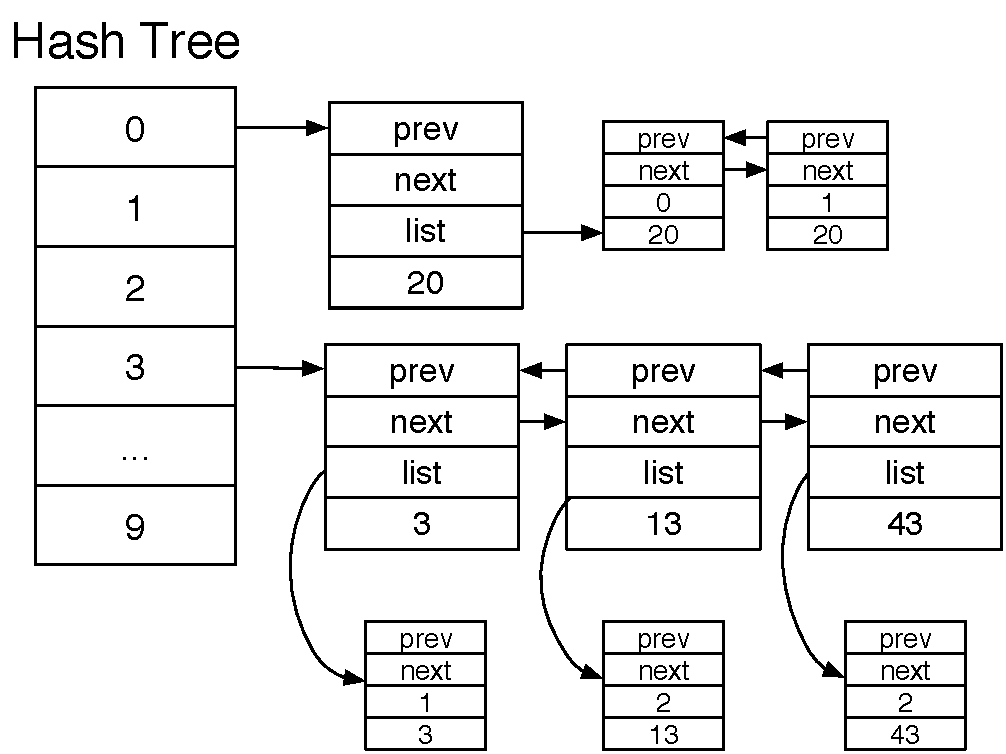
\includegraphics[width=0.6\textwidth]{figures/implementation/hash_table.pdf}
\caption{Hash table and doubly linked data structures for 
   a \texttt{a(int,int)} predicate.}
\label{fig:implementation:hash_table}
\end{figure}

\subsubsection{Locking}

Each node is protected by a main spin-lock that allows threads to change node
attributes. There is also a database spin-lock that protects the internal
database of the node and is locked whenever the node is in the \textbf{working}
state.  

To avoid unnecessary copying, when a node sends facts to a node located in
another thread, the current thread first attempts to lock the database lock of
the target node in order to directly update its database and indexing
structures, otherwise it adds the facts to the list of incoming facts that are
later processed by the owner thread of the target node.


%%%%%%%%%%%%%%%%%%%%%%%%%%%%%%%%%%%%%%%%%%%%%%%%%%%%%%%%%%%%%%%%%%%%%%

\subsection{Rule Engine}
\label{sec:implementation:rule_engine}

The rule engine decides which rules may need to be executed while taking into
account rule priorities. To understand how our engine works, consider the
following set of facts and rules:

\begin{Verbatim}[numbers=left]
a, e(1) -o b.  // rule 1
a -o c.        // rule 2
b -o d.        // rule 3
e(0) -o f.     // rule 4
c -o e(1).     // rule 5

a.
e(0).
\end{Verbatim}

Figure~\ref{fig:implementation:rule_engine} shows the rule engine data
structures for this example. The purpose of each data structure is as follows:

\begin{itemize}

   \item \texttt{Rule Queue} is the bitmap representing the rules scheduled to
      run. The $i^{th}$ is set if the $i^{th}$ rule is scheduled to run;

   \item \texttt{Rule Counter}, which keeps a count of the number of predicates
      needed by the rule that exist in the database. For the rule
      \texttt{a, e(1) -o b} then the rule needs predicates \texttt{a} and
      \texttt{e} and the rule counter is at the most 2 (where the rule can be
      executed).

   \item \texttt{Predicate Bitmap} is a bitmap representing the existence of a
      given predicate in the database;

\end{itemize}

\begin{figure}[t]
   \centering
   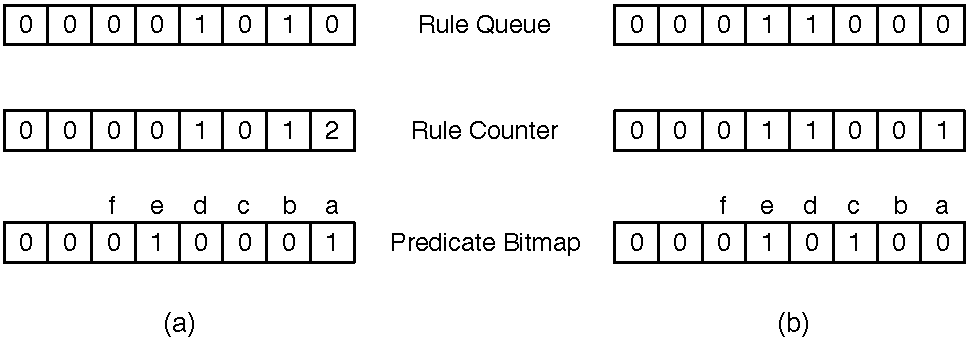
\includegraphics[width=0.8\textwidth]{figures/implementation/rule_queue.pdf}
   \caption{Rule engine data structures (a) before and (b) after applying 
      the rule \texttt{a -o c}.}
   \label{fig:implementation:rule_engine}
\end{figure}

Since we have facts for predicates \texttt{a} and \texttt{e}, the \texttt{Rules
Counter} starts with rules 1, 2 and 4 with 2, 1, 1 predicate counts. Since these
rules have the required counter to be applied, the \texttt{Rule Queue} bitmap
starts with the same three rules.  In order to pick rules for execution, we take
the rule corresponding to the least significant bit from the \texttt{Rule Queue}
bitmap, initially the first rule \texttt{a, e(1) -o b}. However, since we don't
have fact \texttt{e(1)}, this rule fails and its bit in \texttt{Rule Queue} must
be set to 0.  Figure~\ref{fig:implementation:rule_engine}(a) shows the rule
engine data structures at that point.

The next rule in \texttt{Rule Queue} is the second rule \texttt{a -o c}.
Because the this rule will succeed, we must consume fact \texttt{a} and derive
fact \texttt{c}. We thus update \texttt{Predicates Bitmap} accordingly, decrease
the counters for the first and second rule in \texttt{Rule Counter} since such
rules are no longer applicable (\texttt{a} was consumed), and increase the
counter for the fifth rule since \texttt{c} was derived. Finally, to update the
\texttt{Rule Queue}, we must schedule the fifth rule since its counter has been
increased to the required number (we have all predicates).  In the continuation,
the rule engine will schedule the fourth and fifth rules to run.
Figure~\ref{fig:implementation:rule_engine}(b) shows the rule engine data
structures at that point.

Note that every node in the program has the same set of data structures
presented in Fig.~\ref{fig:implementation:rule_engine}. We use 64 bit integers
to implement the 2 bitmaps and an array of 16 bits integers for \texttt{Rule
Counter}.

We do a small optimization to reduce the number of derivations of persistent
facts and, for that, we divide the program rules into two sets: \emph{persistent
rules} and \emph{non persistent rules}. Persistent rules are rules where only
persistent facts are involved. We compile such rules incrementally, i.e., we
attempt to fire all rules where a persistent fact is used. This is called the
\emph{pipelined semi-naive} evaluation and it originated in the P2
system~\cite{Loo-condie-garofalakis-p2}. This evaluation method avoids excessing
re-derivations of the same fact. The order of derivation does not matter for
those rules, since only persistent facts are used.

\subsection{Indexing}\label{sec:implementation:indexing}

To improve fact lookup, the VM employs a fully dynamic mechanism to
decide which argument may be optimal to index.  The algorithm is
performed in the beginning of execution and empirically tries to
assess the argument of each predicate that more equally spreads the
database across the values of the argument.  A single thread performs
the algorithm for all predicates.

The indexing algorithm is performed in three main steps. First, it
gathers lookup statistics by keeping a counter for each
predicate's argument.  Every time a fact search is performed where
arguments are fixed to a value, the counter of such arguments is
incremented. This phase is performed during rule execution for a small
fraction of the nodes in the program.

The second step of the algorithm selects the candidate arguments of each
predicate.  If a predicate was not searched with any fixed arguments, then it
will be not indexed and there are no candidates.  If only one argument was
fixed, then such argument is the only available candidate argument and thus
immediatelly becomes the indexing argument. Otherwise, the top 2 arguments are
selected for the third phase, where \emph{entropy statistics} are collected
dynamically.

During the third phase, each candidate argument has an entropy score.
Before a node is executed, the facts of the target predicate
are used in the following formula applied for the two arguments:

\[
Entropy(A, F) = - \sum_{v \in values(F, A)} \frac{count(F, A = v)}{total(F)} \log_2 \frac{count(F, A = v)}{total(F)}
\]

\noindent where $A$ is the target argument, $F$ is the set of linear facts for
the target predicate, $values(F, A)$ is set of values of the argument $A$,
$count(F, A = v)$ counts the number of linear facts where argument $A$ is equal
to $v$ and $total(F)$ counts the number of linear facts in $F$.  The entropy
value is a good metric because it tells us how much information is needed to
describe an argument. If more information is needed, then that must be the best
argument to index.

For one of the arguments to score, $Entropy(A, F)$ multiplied by the number of
times it has been used for lookup, must be larger than the other argument. The
argument with the best score is selected and then a global variable called
\texttt{indexing\_epoch} is updated. In order to convert the node's linked lists
into hash tables, each node also has a local variable called
\texttt{indexing\_epoch} that is compared to the global variable in order to
rebuild the database according to the new indexing information.

The VM also dynamically resizes the hash table if necessary. When the hash table
becomes too dense, it is doubled in size. When it becomes too sparse, it is
reduced in half or simply transformed back into a doubly linked list. This is
done once in a while, before a node executes.

We have seen very good results with this scheme. The overhead of dynamic
indexing is negligible since programs run almost as fast as if the indices have
been added from the start. However, the programmer can still index predicates
statically, if needed.


\section{Compilation}
As an intermediate step, our compiler first transforms rules into high level
instructions that are then transformed into C++. In Appendix~\ref{appendix:vm}
we present an overview of the high level instructions that can be used as a
reference to the operations that are required by the compiler. In this section,
we present the main algorithm of the compiler and its key optimizations. To make
our presentation more readable, we present our examples using pseudo-code
instead of C++ code.

\subsection{Ordinary Rules}\label{sec:compile}

After a rule is compiled, it must respect the \emph{fact constraints}
(facts must exist in the database) and the \emph{join constraints} that can be
represented by variable constraints and/or boolean expressions. For instance,
consider the second rule of the bipartiteness checking program presented in
Fig.~\ref{language:code:bichecking}:

\begin{Code}
visit(A, P),
colored(A, P)
   -o colored(A, P).
\end{Code}

The fact constraint include the facts required to trigger the rule, namely
\code{visit(A, P)} and \code{colored(A, P)}, and the join constraints include
the implicit constraint that the second argument of \code{visit} must be equal
to the second argument of \code{colored} because the variable \code{P} is used
for both arguments. However, rules may also have explicit constraints, such as:

\begin{Code}
visit(A, P1),
colored(A, P2),
P1 <> P2
   -o fail(A).
\end{Code}

The data structures presented in Section~\ref{sec:data_structures} support
iteration over facts and for linear facts, they also support deletion. Iteration
is provided through \emph{iterators}. For linked lists, the iterator points to
the linear fact in the list and uses the \code{next} field to traverse the list.
For hash tables, it is possible to iterate through the whole table or iterate
through a single bucket. For tries, while iteration goes through every fact, the
operation can be customized with join constraints in order to prune search. To
illustrate how rules are compiled, consider again the rule:

\begin{Code}
visit(A, P),
colored(A, P)
   -o colored(A, P).
\end{Code}

The compiler transforms the rule into two nested \emph{while} loops, as follows:

\begin{LineCode}
colored_list <- linked_list("colored")
visit_list <- linked_list("visit")
visit <- visit_list.head()
while(visit is valid)
{
   colored <- colored_list.head() // Retrieve first element of the list.
   while(colored is valid)
   {
      if(visit.get_int(1) == colored.get_int(1)) { // Equal arguments?
         // New fact is derived.
         new_colored <- create_fact("colored") // New fact for predicate colored.
         new_colored.set_int(1, visit.get_int(1)) // Set arguments.

         colored_list.add(new_colored) // Add new fact to the linked list.

         // Deleting used up facts.
         colored <- colored_list.delete_and_next(colored)
         visit <- visit_list.delete_and_next(visit)
         goto next
      }
      colored <- colored.next()
   }
   visit <- visit.next()
next:
   continue
}
\end{LineCode}

The compilation algorithm iterates through the atomic propositions of the rule's
LHS and creates nested loops to try all the possible combinations of facts.  For
this rule, all the pairs of facts \code{colored} and \code{visit} must be
searched until the implicit constraint is true. First, the \code{visit} linked
list is iterated over by first retrieving the head fact and then using the
\code{next} pointer of each fact. Inside this outer loop, a nested \code{while}
loop is created for predicate \code{colored}. This inner loop includes a check
for the constraint.

If the constraint expression is true then the rule matches and a new
\code{colored} fact is derived and two used linear facts are consumed by
deleting them from the linked lists. After the rule is derived, the \code{visit}
and \code{colored} facts are deleted from the linked list and the pointers
adjusted to the next elements of each list. Afterwards, the \code{goto next}
statement is used to jump to the outer loop, which will use the new fact
pointers. This forces the procedure to try all the combinations of the rule from
the database.  Furthermore, we must jump to the first linear loop because we
cannot use the next fact from the deepest loop since we may have constraints
between the first linear loop and the deepest loop that were validated using
deleted facts.

If the implicit constraint failed, another \code{colored} fact would be checked
by assigning \code{colored} to \code{colored.next()}.  Likewise, if the initial
\code{visit} fact fails for all \code{colored} facts, then the next
\code{visit} fact in the list is tried by following the \code{next} pointer.

In order to understand how rule priorities affect compilation, consider a
slightly different bipartiteness checking program where the second and third
rules are swapped:

\begin{LineCode}[commandchars=\*\[\]]
visit(A, P),
uncolored(A)
   -o {B | !edge(A, B) -o visit(B, next(P))},
      colored(A, P).

visit(A, P1),
colored(A, P2),
P1 <> P2
   -o fail(A).*label[line:implementation:higher]

*textbf[visit(A, P),]
*textbf[colored(A, P)]
   *textbf[-o colored(A, P).]

visit(A, P),
fail(A)
   -o fail(A).
\end{LineCode}

The procedure for the rule being compiled cannot be the same since the derived
\code{colored} fact is used in the LHS of a higher priority rule, namely, the
rule in line~\ref{line:implementation:higher}. Once the \code{colored} fact is
derived, the procedure must return to schedule the higher priority rule, as
follows:

\begin{LineCode}[commandchars=\$\#\&]
colored_list <- linked_list("colored")
visit_list <- linked_list("visit")
colored <- colored_list.head()
while(colored is valid)
{
   visit <- visit_list.head() // Retrieve first element of the list.
   while(visit is valid)
   {
      if(visit.get_int(1) == colored.get_int(1)) { // Equal arguments?
         new_colored <- create_fact("colored") // New fact for predicate colored.
         new_colored.set_int(1, visit.get_int(1)) // Set arguments.

         // New fact is derived.
         colored_list.add(new_colored) // Add new fact to the linked list.

         // Deleting facts.
         colored_list.delete_and_next(colored)
         visit_list.delete_and_next(visit)
         $textbf#return&
      }
      visit <- visit.next()
   }
   colored <- colored.next()
}
\end{LineCode}

This enforces the priority semantics of the language described in
Section~\ref{sec:language:semantics}. When a rule derives facts
that were used as input to a higher priority rule, the initial rule is only
derived once because the newly derived facts may trigger the derivation of a
higher priority rule.
    
\begin{figure}
\begin{algorithm}[H]
 \KwData{Rule R1, Rules}
 \KwResult{Compiled Code}
 $LHSProps \longleftarrow LHSAtomicPropositionsFromRule(R1)$\;
 $Constraints \longleftarrow ConstraintsFromRule(R1)$\;
 $Code \longleftarrow CreateFunctionForRule()$\;
 $FactIterators \longleftarrow []$\;
 $CompiledProps = []$\;
 \While{$LHSProps$ not empty}{
  $Prop \longleftarrow RemoveBestProposition(LHSProps)$\;
  $CompiledProps.push(Prop)$\;
  $Iterator \longleftarrow Code.InsertIteration(Prop)$\;
  $FactIterators.push(Iterator)$\;
  \tcp{Select constraints that are covered by CompiledFacts.}
  $NextConstraints \longleftarrow RemoveConstraints(Constraints, CompiledProps)$\;
  $Code.InsertConstraints(NextConstraints)$\;
 }
 $RHSProps = RHSAtomicPropositionsFromRule(R1)$\;
 \While{$RHSProps$ not empty}{
    $Prop \longleftarrow RemoveFact(RHSProps)$\;
    $Code.InsertDerivation(Prop)$\;
 }
 \For{$Iterator \in FactIterators$}{
    \If{$IsLinear(Iterator)$}{
       $Code.InsertRemove(Iterator)$\;
    }
 }
 \tcp{Enforce rule priorities.}
 \uIf{$FactsDerivedUsedBefore(Rules, R1)$}{
    $Code.InsertReturn()$\;
 }
 \Else{
    $Code.InsertGoto(FirstLinear(FactIterators))$\;
 }
 \Return{$Code$}
\end{algorithm}
 \mycap{Compiling LM rules into C++ code.}
 \label{alg:compile_rule}
\end{figure}

Figure~\ref{alg:compile_rule} presents the algorithm for compiling rules into
C++ code. First, we split the rule's RHS into atomic propositions and
constraints. Fact expressions map directly to iterators while fact constraints
map to \emph{if} expressions. A possible compilation strategy is to first
compile all the atomic propositions and then compile the constraints. However,
this may require unneeded database lookups since some constraints may fail
early.  Therefore, our compiler introduces constraints as soon as all the
variables in the constraint are all included in the already compiled atomic
propositions. The order in which fact propositions are selected for compilation
does not interfere with the correctness of the compiled code, thus our compiler
selects the atomic proposition ($RemoveBestProposition$) that needs the highest
number of join constraints, in order to prune search and avoid undesirable
database lookups. If two atomic propositions have the same number of new
constraints, then the compiler always picks the persistent proposition since
persistent facts are not deleted.

Derivation of new facts belonging to the local node requires only that the new
facts are added to the local node data structure. Facts that belong to other
nodes are sent using an appropriate runtime API.

\subsection{Persistence Checking}

Not all linear facts need to be deleted. For instance, in the compiled rule
above, the fact \code{colored(A, P)} is re-derived in the rule's RHS.  Our
compiler is able to turn linear loops into persistent loops for linear facts
that are consumed and then asserted. The rule is then compiled as follows:

\begin{LineCode}[commandchars=\$\#\&]
colored_list <- linked_list("colored")
visit_list <- linked_list("visit")
colored <- colored_list.head()
while(colored is valid)
{
   visit <- visit_list.head() // Retrieve first element of the list.
   while(visit is valid)
   {
      if(visit.get_int(1) == colored.get_int(1)) { // Equal arguments?
         // Delete visit.
         visit <- visit_list.delete_and_next(visit) // Get next visit fact.
         goto next$label#line:implementation:goto&
      }
      visit <- visit.next()
$textbf#next:&
      $textbf#continue&
   }
   colored <- colored.next()
}
\end{LineCode}

In this new version of the code, only the \code{visit} facts are deleted, while
the \code{colored} facts remain untouched. In the bipartiteness checking
program, each node has one \code{colored} fact and this compiled code simply
filters out the \code{visit} facts with the same color. Please note that the
\code{colored} facts are now iterated in the outer loop in order to make the
\code{goto} statement jump to the inner loop. This is now possible because the
\code{colored} fact is not deleted during rule derivation.

\subsection{Updating Facts}

Many inference rules consume and then derive the same predicate but with
different arguments. The compiler recognizes those cases and, instead of
consuming the fact from its linked list or hash table, it updates the fact
in-place. As an example, consider the following rule:

\begin{Code}
new-neighbor-pagerank(A, B, New),
neighbor-pagerank(A, B, Old)
   -o neighbor-pagerank(A, B, New).
\end{Code}

Assuming that \code{neighbor-pagerank} is stored in a hash table and indexed by
the second argument, the code for the rule above is as follows:

\begin{LineCode}
new_neighbor_pagerank_list <- linked_list("new-neighbor-pagerank")
neighbor_pagerank_table <- hash_table("neighbor-pagerank")
new_neighbor_pagerank <- new_neighbor_pagerank.head()
while(new_neighbor_pagerank is valid)
{
   // Hash table for neighbor-pagerank is indexed by the second argument,
   // therefore we search for the bucket using the second argument
   // of new-neighbor-pagerank.
   neighbor_pagerank <- neighbor_pagerank_table.lookup(new_neighbor_pagerank.get_node(1))
   while(neighbor_pagerank is valid)
   {
      if(new_neighbor_pagerank.get_node(1) == neighbor_pagerank.get_node(1))
      {
         // Update fact argument.
         neighbor_pagerank.set_float(2, new_neighbor_pagerank.get_float(2))
         new_neighbor_pagerank <- new_neighbor_pagerank_list.
                  delete_and_next(new_neighbor_pagerank)
         goto next
      }
      neighbor_pagerank <- neighbor_pagerank.next()
   }
   new_neighbor_pagerank <- new_neighbor_pagerank.next()
next:
   continue
}
\end{LineCode}

Note that \code{neighbor-pagerank} fact is updated using \code{set\_float}. The
rule also does not return since it is the highest priority rule. If there was a
higher priority rule using \code{neighbor-pagerank}, then the code would have to
return since the act of updating a fact is equivalent to deriving a new one.

\subsection{Enforcing Linearity}

We have already introduced the \code{goto} statement as a mechanism to avoid
reusing deleted linear facts. However, this is not enough in order to enforce
linearity of facts. Consider the following inference rule:

\begin{Code}
add(A, N1),
add(A, N2)
   -o add(A, N1 + N2).
\end{Code}

Using the standard compilation algorithm, two nested loops are created, one for
each \code{add} fact. However, notice that there is an implicit constraint (the
two \code{add} linear facts must be different) when creating the iterator for
\code{add(A, N2)} since this fact cannot be the same as the first one. That
would invalidate linearity since a single linear fact would be used to prove two
linear facts. This is easily solved by adding a constraint in the inner loop by
checking if the second fact is the same as the first one.

\begin{LineCode}
add_list <- linked_list("add")
add1 <- add_list.head()
while(add1 is valid)
{
   add2 <- add_list.head()
   while(add2 is valid)
   {
      if(add1 != add2)
      {
         add1.set_int(1, add1.get_int(1) + add2.get_int(1))
         add2 <- add_list.delete_and_next(add2)
         goto next
      }
      add2 <- add2.next()
   }
   add1 <- add1.next()
next:
   continue
}
\end{LineCode}

Figure~\ref{fig:local:update_add} presents the steps for executing this rule
when the database contains three facts. The fact variables never point to the
same fact.

\begin{figure}
\centering
\begin{minipage}{.5\textwidth}
  \centering
  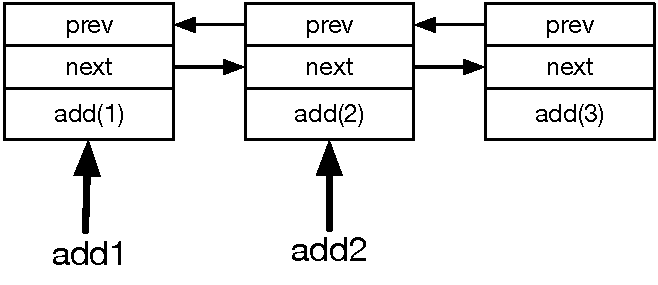
\includegraphics[width=.8\linewidth]{figures/compiler/update}
\end{minipage}%
\begin{minipage}{.5\textwidth}
  \centering
  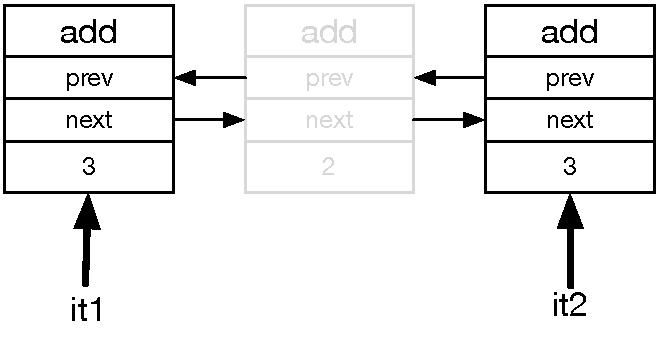
\includegraphics[width=0.8\linewidth]{figures/compiler/update2}
\end{minipage}
\begin{minipage}{.5\textwidth}
   \centering
   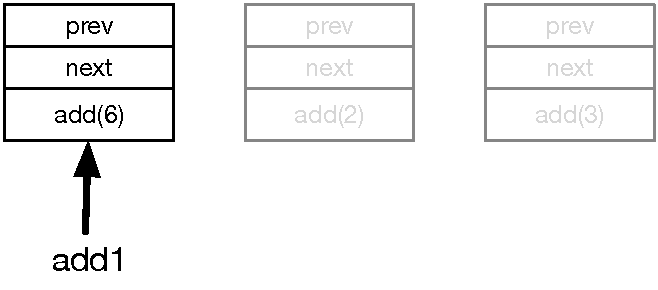
\includegraphics[width=0.8\linewidth]{figures/compiler/update3}
\end{minipage}
\mycap{Executing the add rule. First, the two iterators point to
   the first and second facts and the former is updated while the latter is
   consumed. The second iterator then moves to the next fact and the first fact is
   updated again, now to the value \code{6}, the expected result.}
\label{fig:local:update_add}
\end{figure}

\subsection{Comprehensions}

Consider the comprehension used in the first rule of the bipartiteness checking
program in Fig.~\ref{language:code:bichecking}:

\begin{Code}
visit(A, P),
uncolored(A)
   -o {B | !edge(A, B) -o visit(B, next(P))},
      colored(A, P).
\end{Code}

The attentive reader will remember that comprehensions are sub-rules, therefore
they should be compiled like normal rules. Comprehensions must also derive all
possible combinations. However, the rule itself must return if the
comprehension's RHS derives a fact that is used by a higher priority rule. The
example rule does not need to return since it has the highest priority and the
\code{visit} facts derived in the comprehension are contained in other nodes.
The code for the rule is shown below:

\begin{LineCode}
colored_list <- linked_list("colored")
visit_list <- linked_list("visit")
uncolored_list <- linked_list("uncolored")
visit <- visit_list.head()
while(visit is valid)
{
   uncolored <- uncolored_list.head()
   while(uncolored is valid)
   {
      // Comprehension code.
      edge_trie <- trie("edge")
      edge <- edge_trie.first()
      while(edge is valid)
      {
         new_visit <- create_fact("visit") // New visit fact.
         new_visit.set_int(1, next(visit.get_int(1)))
         // Send fact to B.
         send_fact(new_visit, edge.get_node(1))
         edge <- edge.next()
      }
      new_colored <- create_fact("colored")
      new_colored.set_int(1, visit.get_int(1))
      colored_list.add(new_colored)
      visit <- visit_list.delete_and_next(visit)
      uncolored <- uncolored_list.delete_and_next(uncolored)
      goto next
   }
   uncolored <- uncolored.next()
next:
   continue
}
\end{LineCode}

Special care must be taken when the comprehension's sub-rule uses the same
predicates that are derived by the main rule. Rule inference must be atomic in
the sense that, after a rule matches, the comprehensions in the rule's RHS can
use the facts that were present before the rule was matched. Consider a rule
with $n$ comprehensions or aggregates, where each $CLHS_i$ and $CRHS_i$ are the
LHS and RHS of the comprehension/aggregate $i$, respectively, and $RHSP$
represents the atomic propositions found in rule's RHS. The formula used by the
compiler to detect conflicts between predicates is the following:

\[
\bigcup^{n}_i[CLHS_i \cap RHSP] \cup \bigcup^{n}_i [CLHS_i \cap \bigcup^{n}_j[CRHS_j]]
\]

If the result of the formula is not empty, then the compiler disables
optimizations for the conflicting predicates and derives the corresponding facts
into a temporary data structure before being added into the database data
structures. As an example, consider the following rule:

\begin{Code}
update(A),
!edge(A, B)
   -o {P | points(A, B, P) -o update(B)},
      points(A, B, 1).
\end{Code}

We have $n = 1$ comprehensions, where $CLHS_0 = $ \code{points(A, B, P)},
$CRHS_0 =$ \code{update(B)}, and $RHSP = $ \code{points(A, B, 1)}. There is a
conflict because $CLHS_0 \cap RHSP = \{\mathtt{points}\}$, which requires
\code{points(A, B, 1)} to be derived after the comprehension or be stored in a
temporary data structure to avoid conflicts with the comprehensions, which could
consume the newly derived fact. Fortunately, most rules in LM programs do not
show these kinds of conflicts and thus can be fully optimized.

\subsection{Aggregates}

Aggregates are similar to comprehensions. They are also sub-rules but a value is
accumulated for each combination of the sub-rule. After all the combinations are
derived, a final RHS term is derived with the accumulated value. Consider the
following rule that computes a PageRank value by aggregating all neighbors
PageRank values:

\begin{Code}
update(A),
pagerank(A, OldRank)
      -o [sum => V; B | neighbor-pagerank(A, B, V) -o neighbor-pagerank(A, B, V)
            -> pagerank(A, damping/P + (1.0 - damping) * V)].
\end{Code}

The variable \code{V} is initialized to \code{0.0} and sums all the PageRank
values of the neighbors as seen in the code below. The aggregate value is then
used to update the second argument of the initial \code{pagerank} fact.

\begin{LineCode}
pagerank_list <- linked_list("pagerank")
update_list <- linked_list("update")
neighbor_pagerank_list <- linked_list("neighbor_pagerank_list")
pagerank <- pagerank_list.head()
while(pagerank is valid)
{
   update <- update_list.head()
   while(update is valid)
   {
      V <- 0.0
      neighbor_pagerank <- neighbor_pagerank_list.head()
      while(neighbor_pagerank is valid)
      {
         V <- V + neighbor_pagerank.get_float(2)
         neighbor_pagerank <- neighbor_pagerank.next()
      }
      // RHS of the aggregate
      pagerank.set_float(1, damping / P + (1.0 - damping) * V)
      update <- update_list.delete_and_next(update)
      goto next
   }
   pagerank <- pagerank.next()
next:
   continue
}
\end{LineCode}



\section{Summary}

This section provided a full description of the implementation of LM, including
its compiler and virtual machine. We explained how the virtual machine is
organized to provide scalable multi threaded execution and fast fact assertion
and retraction using efficient data structures. We also gave a detailed
description of the compilation algorithm used to transform LM rules into
efficient C++ code.
